
\section*{Introduction}

Seasonal influenza virus infects 5--15\% of the global population every year causing an estimated 250,000 to 500,000 deaths annually \cite{flufactsheet}.
Vaccination remains the most effective public health response available.
However, frequent viral mutation results in viruses that escape previously acquired human immunity.
The World Health Organization (WHO) selects vaccine viruses to match circulating viruses, but because the process of vaccine development and distribution requires several months to complete, accurate vaccine strain selection requires a prediction of which viruses will predominate approximately one year after vaccine viruses are selected.
Current vaccine predictions focus on the hemagglutinin (HA) protein, which acts as the primary target of human immunity.
The hemagglutination inhibition (HI) assay \cite{hirst1943studies} is used to measure the degree of cross-reactivity between pairs of circulating viruses.
HI assays are fundamental for vaccine strain selection, but they are laborious and low-throughput compared to genome sequencing \cite{Wood:2012ii}.
As a result, researchers have developed computational methods to predict influenza fitness from sequence data alone \cite{Luksza:2014hj,Steinbruck:2014kq,Neher:2014eu}.

Despite the promise of these sequence-only models, they explicitly omit experimental measurements of antigenic or functional phenotypes.
Recent developments in computational methods and influenza virology have made it feasible to integrate these important metrics of influenza fitness into a single predictive model.
For example, phenotypic measurements of antigenic drift are now accessible through phylogenetic models \cite{Neher:2016hy} and functional phenotypes for HA are available from deep mutational scanning experiments \cite{Lee2018}.
We describe an approach to integrate previously disparate sequence-only models of influenza evolution with high-quality experimental measurements of antigenic drift and functional constraint.

The influenza community has long recognized the importance of incorporating HI phenotypes and other experimental measurements of viral phenotypes with existing forecasting methods into an extensible, open source framework that can be used by professional virologists in their vaccine design process \cite{Gandon:2016gz,Morris:2017ea,Lassig:2017hr}.
Although several distinct efforts have made progress in using HI phenotypes to evaluate the evolution of seasonal influenza \cite{Steinbruck:2014kq,Neher:2016hy}, these methods stop short of developing a complete forecasting framework wherein the evolutionary contribution of HI phenotypes can be compared and contrasted with new and existing fitness metrics.
Here, we provide the first such open source long-term forecasting framework for seasonal influenza.
With this framework, we show that HI phenotypes enable more accurate long-term forecasts of A/H3N2 populations compared to previous metrics based on epitope mutations alone.
However, we also find that phylogenetic fitness metrics based on recent growth of circulating clades consistently outperform any combination of genotypic or phenotypic metrics, suggesting that existing mechanistic models of seasonal influenza evolution are missing critical components.

\section*{Results}

\subsection*{A distance-based model of seasonal influenza evolution}

\begin{figure*}[ht]
  \begin{center}
  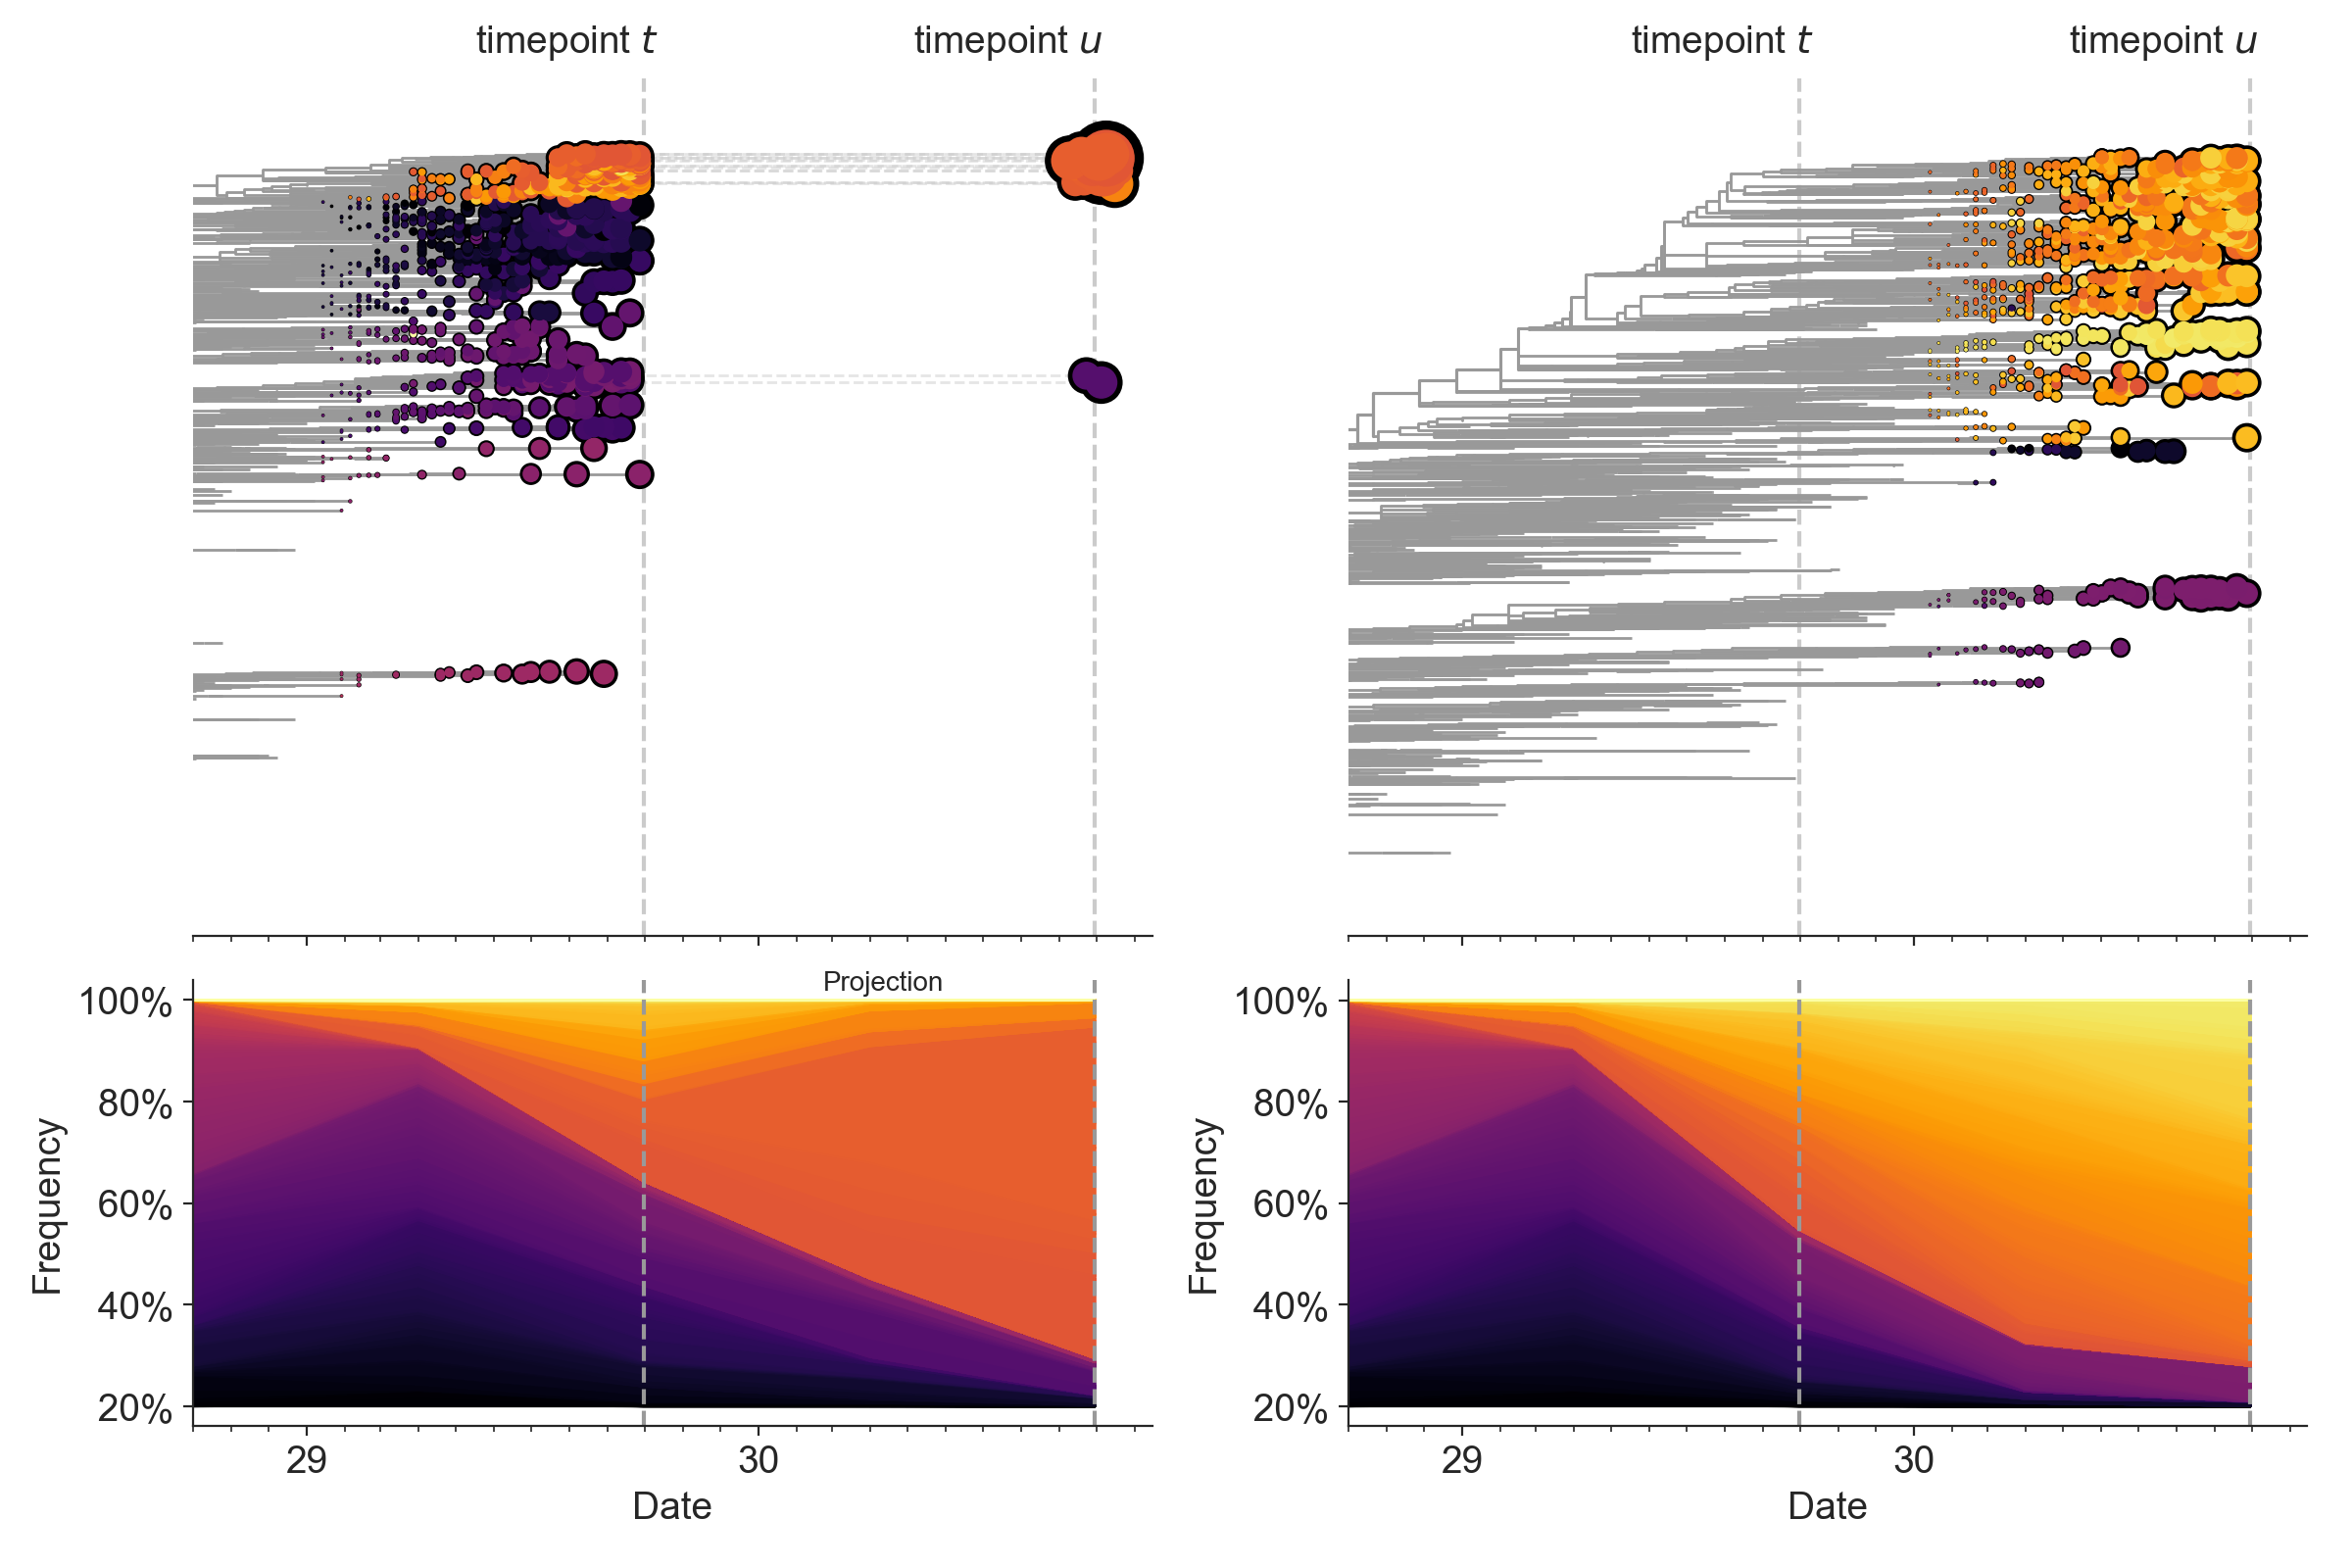
\includegraphics[width=\columnwidth]{figures/distance-based-fitness-model.png}
  \caption{
    Schematic representation of the fitness model for simulated A/H3N2-like populations wherein the fitness of samples at timepoint $t$ determines the estimated frequency of samples with similar sequences one year in the future at timepoint $u$.
    Samples are colored by their amino acid sequence composition such that genetically similar samples have similar colors.
    A) Samples at timepoint $t$ are shown in their phylogenetic context and sized by their frequency at that timepoint.
    The estimated future population at timepoint $u$ is projected to the right with samples scaled in size by their projected frequency based on the true fitness model.
    B) The frequency trajectories of samples at timepoint $t$ to $u$ represent the predicted the growth of the orange samples to the detriment of the purple samples.
    C) Samples at timepoint $u$ are shown in the corresponding phylogeny for that timepoint and scaled by their frequency at that time.
    D) The observed frequency trajectories of samples at timepoint $u$ broadly recapitulate the model's forecasts while also revealing increased diversity of sequences at the future timepoint that the model could not anticipate, e.g. the emergence of the yellow cluster from within the successful orange cluster.
  }
  \label{fig:model}
  \end{center}
\end{figure*}

Here, we present a model of seasonal influenza evolution inspired by the Malthusian growth fitness model of {\L}uksza and L\"assig \cite{Luksza:2014hj}.
As with this original model, we seek to forecast the frequencies of viral populations one year in advance by applying to each virus sample an exponential growth factor scaled by an estimate of the sample's fitness (Fig.~\ref{fig:model} and Eq.~\ref{equation_exponential_growth_model}).
We estimate the frequency of virus samples every six months using a smoothed KDE kernel to represent the frequency of each sample.

We estimate viral fitness with biologically-informed metrics including those originally defined by \cite{Luksza:2014hj} of epitope cross-immunity and non-epitope mutations as well as four more recent metrics including hemagglutination inhibition (HI) cross-immunity \cite{Neher:2016hy}, deep mutational scanning (DMS) mutational effects \cite{Lee2018}, local branching index (LBI) \cite{Neher:2014eu}, and change in clade frequency over time (delta frequency).
All of these metrics except for HI cross-immunity and DMS mutational effects rely only on HA sequences.
The cross-immunity metrics estimate how antigenically distinct each sample at time $t$ is from previously circulating samples based on either genetic distance at epitope sites or HI distance.
The functional constraint metrics consider effects of mutations accumulated since the previous season either for deleterious (non-epitope) mutations or all mutations based on their DMS preferences.
The growth metrics estimate how successful populations of samples have been in the last six months based on either rapid branching in the phylogeny (LBI) or the change in clade frequencies over time (delta frequency).

We fit models by learning coefficients for each fitness metric either individually or in linear combinations from training data and select the best of these models using time-series cross-validation.
After selecting optimal models from training and validation, we evaluated the true out-of-sample errors of these models on additional data that were held out from the initial model fitting and tuning.
Importantly, our models find fitness coefficients that minimize the normalized average Hamming distance between the observed population one year in the future and the estimated population produced by the fitness model (Fig.~\ref{fig:model}).
With this approach, we avoid the intrinsic instability of clade definitions due to variability in phylogenetic reconstruction from year to year.
However, we retain the benefits of fitting models to highly similar samples found within clades and enable future forecasting efforts for pathogens whose sequences are not amenable to standard phylogenetic inference.

\subsection*{Models accurately forecast evolution of A/H3N2-like viruses}

The long-term evolution of influenza A/H3N2 hemagglutinin has been previously described as a balance between positive selection for substitutions that enable escape from adaptive immunity by modifying existing epitopes and purifying selection on domains that are required to maintain the protein's primary functions of binding and membrane fusion \cite{Bush:1999vj,Neher2013,Luksza:2014hj,Koelle:2015dh}.
To test the ability of our models to accurately detect these evolutionary patterns under controlled conditions, we simulated the long-term evolution of A/H3N2-like viruses under positive and purifying selection for 40 years (Methods, Supplemental Figure~\ref{sup_fig:cross_validation_for_simulated_populations}).
These selective constraints produced phylogenetic structures and accumulation of epitope and non-epitope mutations that were consistent with phylogenies of natural A/H3N2 HA (Supplemental Figure \ref{sup_fig:simulated_h3n2_ha_phylogeny}).
We fit models to these simulated populations using all sequence-only fitness metrics.
As a positive control for our model framework, we also fit a model based on the true fitness of each sample as measured by the simulator.
We evaluated the performance of each model relative to the observed distance between timepoints.

We hypothesized that fitness metrics associated with viral success such as epitope cross-immunity, LBI, and delta frequency would be assigned positive coefficients, while metrics associated with fitness penalties, like non-epitope mutations, would receive negative coefficients.
We reasoned that both LBI and delta frequency would individually outperform the mechanistic metrics as both of these growth metrics estimate recent clade success regardless of the mechanistic basis for that success.
Correspondingly, we expected that a composite model of epitope cross-immunity and non-epitope mutations would perform as well as or better than the growth metrics, as this model would include both primary fitness constraints acting on our simulated populations.

\begin{figure*}[ht!]
  \begin{center}
  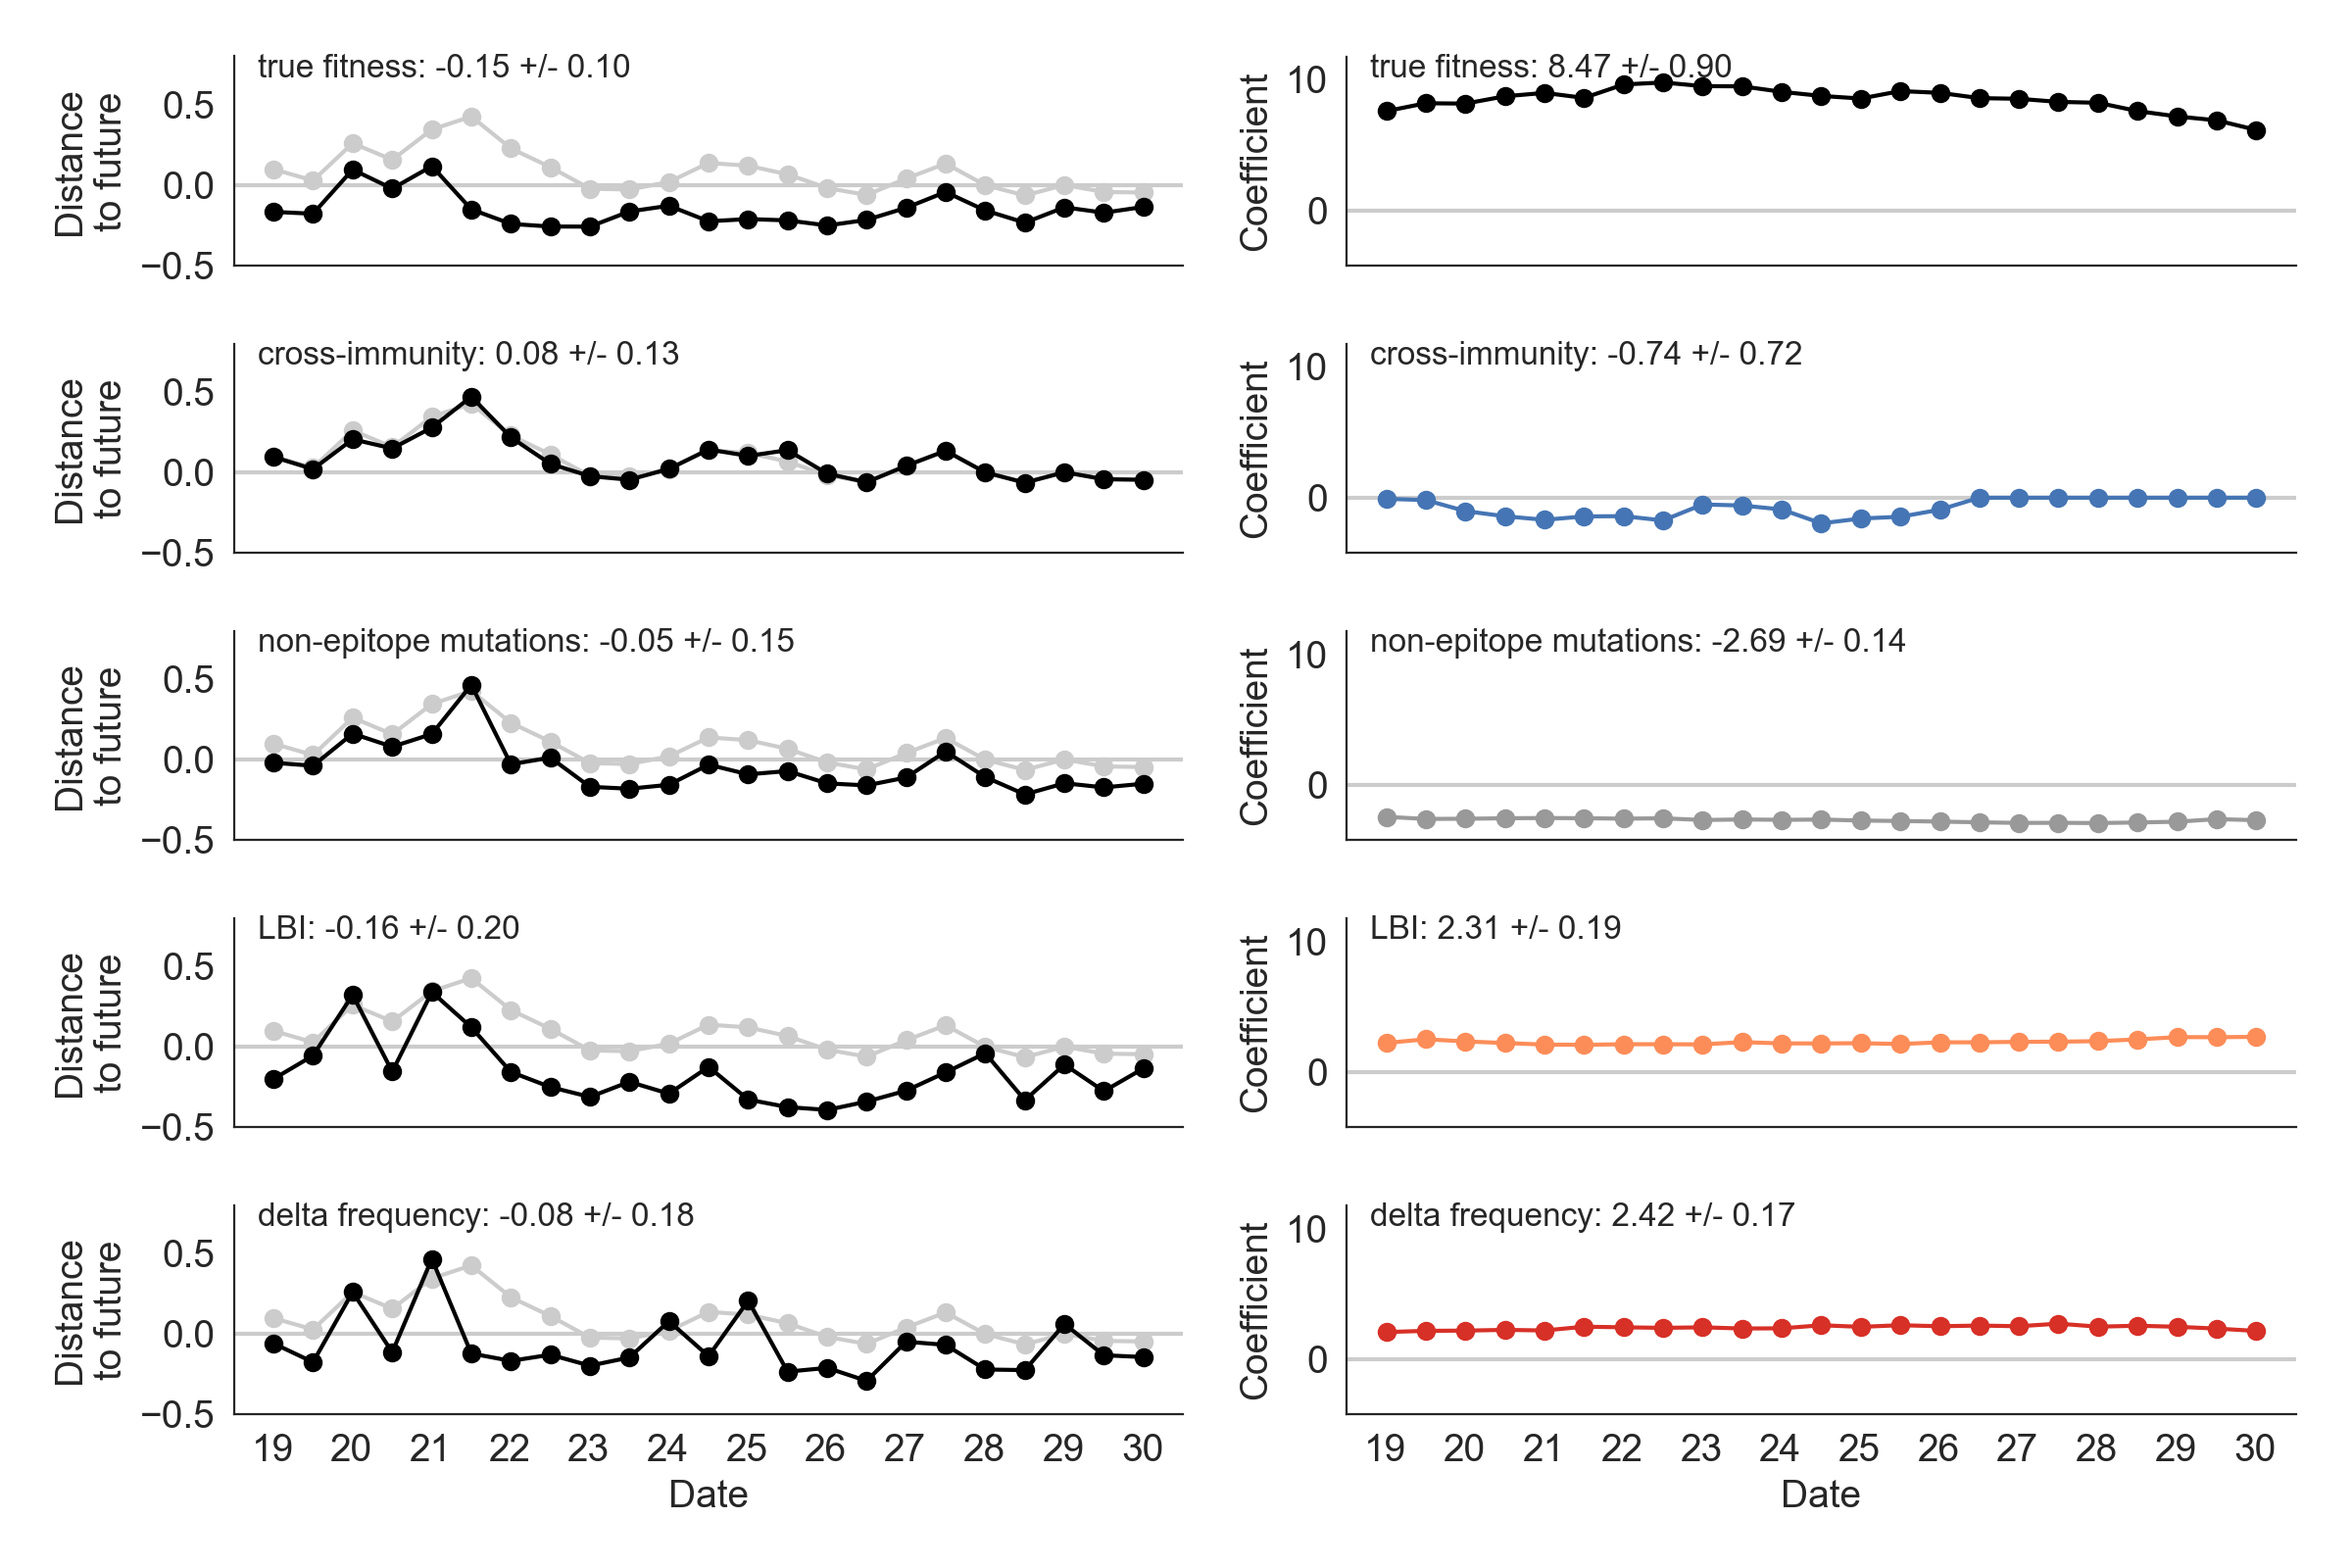
\includegraphics[width=\textwidth]{figures/unadjusted-model-accuracy-and-coefficients-for-simulated-populations.png}
  \caption{
    Model a) coefficients and b) distances closer to the future measured in amino acids (AAs) for each model relative to a naive model for simulated populations.
    Coefficients are shown for each individual fitness metric per validation timepoint (N=33) in solid circles with the mean $\pm$ standard deviation in the top-left corner of each panel.
    Distances closer to the future in amino acids are shown per validation or test timepoint for each individual model relative to the observed distance between timepoints.
    Models outperform the naive model when the distances closer to the future are greater than zero.
    The mean $\pm$ standard deviation of amino acids per validation timepoint are shown in the top-left of each panel.
    The same values are shown per test timepoint in the top-right of each panel.
    Solid circles indicate validation timepoints and open circles indicate test timepoints when coefficients are fixed to their mean values from training/validation and applied to out-of-sample test data.
  }
  \label{fig:unadjusted_model_accuracy_and_coefficients_for_simulated_populations}
  \end{center}
\end{figure*}

\begin{table*}[ht]
  \begin{center}
    
\begin{tabular*}{1.1\textwidth}{lrllrr}
\toprule
        &                 & \multicolumn{2}{c}{Distance to future (AAs)} & \multicolumn{2}{c}{Model $>$ naive} \\
  Model &    \makecell{Coefficients} & \makecell{Validation} & \makecell{Test} & \makecell{Validation} & \makecell{Test} \\
\midrule

true fitness & 9.37 +/- 0.92 & 6.82 +/- 1.52* & 7.38 +/- 1.89* & 32 (97\%) & 16 (89\%) \\
LBI & 1.31 +/- 0.33 & 7.24 +/- 1.66* & 7.10 +/- 1.19* & 32 (97\%) & 18 (100\%) \\
\hspace{5mm} + mutational load & -1.77 +/- 0.49 & & & & \\
LBI & 2.26 +/- 1.06 & 7.57 +/- 1.85* & 7.51 +/- 1.20* & 29 (88\%) & 17 (94\%) \\
delta frequency & 1.46 +/- 0.44 & 8.13 +/- 1.44* & 8.65 +/- 1.99 & 26 (79\%) & 13 (72\%) \\
epitope ancestor & 0.35 +/- 0.07 & 8.20 +/- 1.39* & 8.17 +/- 1.52* & 29 (88\%) & 17 (94\%) \\
\hspace{5mm} + mutational load & -1.57 +/- 0.13 & & & & \\
mutational load & -1.49 +/- 0.12 & 8.27 +/- 1.35* & 8.20 +/- 1.50* & 29 (88\%) & 17 (94\%) \\
epitope antigenic novelty & 0.03 +/- 0.19 & 8.33 +/- 1.35* & 8.22 +/- 1.51* & 28 (85\%) & 17 (94\%) \\
\hspace{5mm} + mutational load & -1.38 +/- 0.39 & & & & \\
epitope ancestor & 0.14 +/- 0.11 & 8.96 +/- 1.35 & 9.03 +/- 1.68 & 20 (61\%) & 13 (72\%) \\
naive & 0.00 +/- 0.00 & 8.97 +/- 1.35 & 9.07 +/- 1.70 & 0 (0\%) & 0 (0\%) \\
epitope antigenic novelty & -0.03 +/- 0.19 & 9.03 +/- 1.37 & 9.07 +/- 1.69 & 14 (42\%) & 7 (39\%) \\

\bottomrule
\end{tabular*}

    \caption{
      Model performance with simulated populations relative to the naive model.
      Models use one or more fitness metrics to minimize the distance between the population of HA amino acid sequences at timepoint, $t$, and those at a timepoint one year in the future, $t + 1$.
      The naive model assumes the populations at time $t$ and $t + 1$ are identical, effectively measuring the observed distance between the two timepoints.
      Better models produce estimates that are closer to the future population than the naive model.
      \tbc{Confused as to why `epitope cross-immunity' isn't working in the simulated example.}
    }
    \label{table_simulated_model_selection}
  \end{center}
\end{table*}

The average distance between yearly populations, as measured by the naive model, was 8.97 $\pm$ 1.35 amino acids (Supplemental Fig.~\ref{sup_fig:distance_of_simulated_populations_between_timepoints}).
\rnc{would be good to compare the year-on-year distance to diversity. that would give some sense whether a 2aa reduction is big or small.}
As expected, the true fitness model outperformed all other models reducing the distance between populations by 2.16 $\pm$ 1.19 amino acids on average and surpassing the naive model in 32 of 33 (97\%) timepoints (Table~\ref{table_simulated_model_selection}).
With the exception of epitope cross-immunity, all biologically-informed models consistently outperformed the naive model (Fig.~\ref{fig:unadjusted_model_accuracy_and_coefficients_for_simulated_populations}).
LBI was the best of these models, reducing the distance between populations by 1.41 $\pm$ 1.30 amino acids on average.
Indeed, both growth-based models received positive coefficients and outperformed the mechanistic models.
The non-epitope mutations metric received a consistently negative coefficient with an average improvement of 0.71 $\pm$ 0.58 amino acids.
Surprisingly, the composite model of epitope cross-immunity and non-epitope mutations did not perform better than the individual non-epitope mutations model (Supplemental Fig.~\ref{sup_fig:unadjusted_composite_model_accuracy_and_coefficients_for_simulated_populations}).
While epitope cross-immunity was not predictive on its own, the consistently positive coefficient it received in the composite model suggested that it was an informative metric.
From these results, we concluded that our method can accurately estimate the evolution of simulated populations, but that the fitness of simulated samples was dominated by purifying selection rather than by positive selection at epitope sites.

We hypothesized that a composite model of mutually beneficial metrics could better approximate the true fitness of simulated viruses than models based on individual metrics.
To this end, we fit an additional model including the best metrics from the mechanistic and clade growth categories: non-epitope mutations and LBI.
This composite model outperformed all individual metrics, reducing the distance between populations by 1.74 $\pm$ 1.02 amino acids and outperforming the naive model as often as the true fitness metric (Fig.~\ref{fig:unadjusted_model_accuracy_and_coefficients_for_simulated_populations}).
The coefficients for LBI and non-epitope mutations remained relatively consistent across all validation timepoints, indicating that these fitness metrics were stable approximations of the simulator's underlying evolutionary processes.
These results support our hypothesis that multiple complementary metrics can produce more accurate models.

\begin{figure*}[ht]
  \begin{center}
  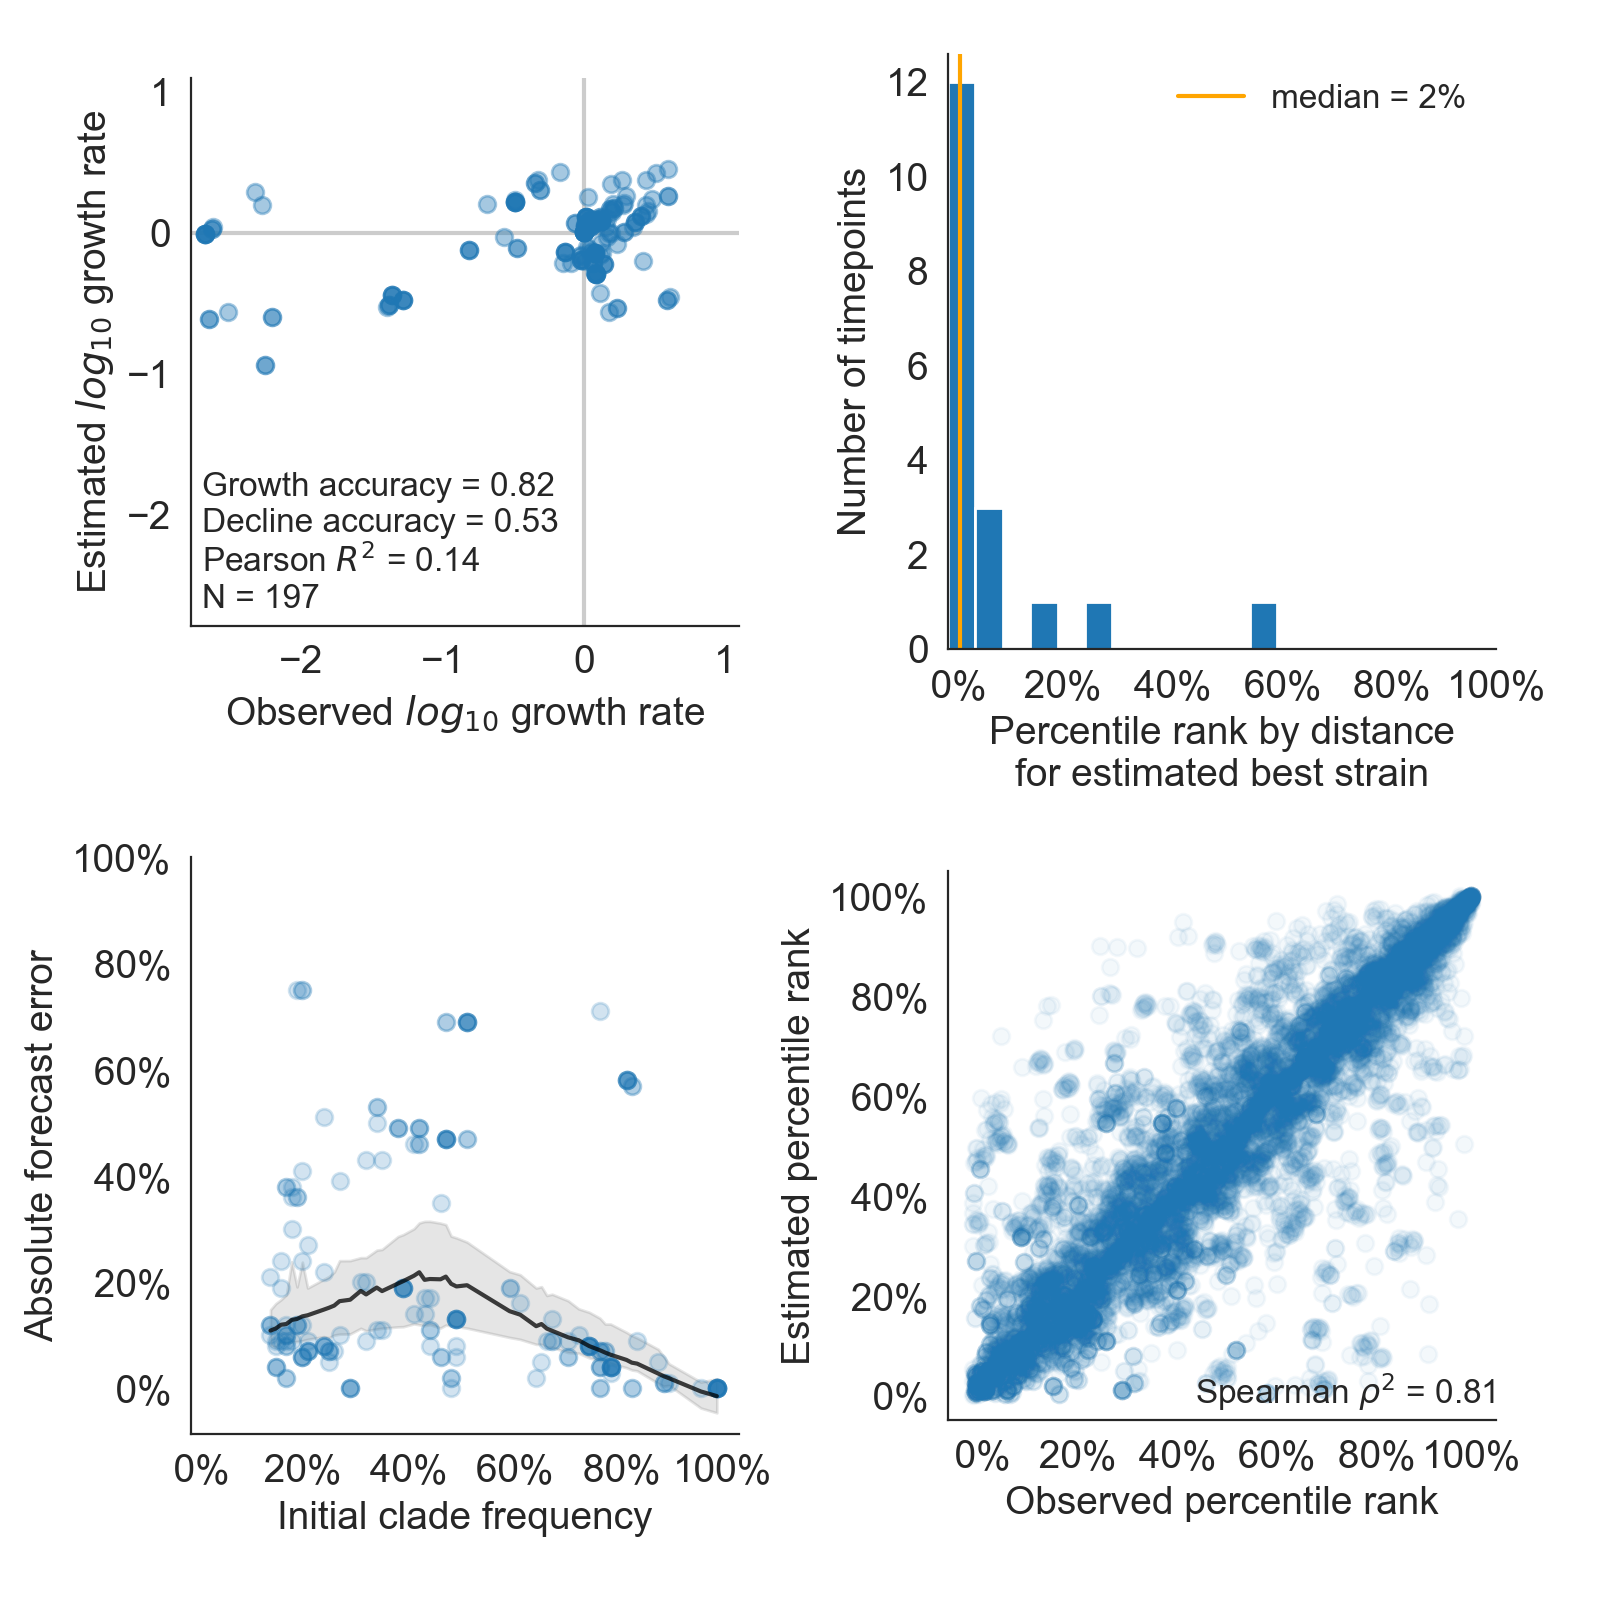
\includegraphics[width=\textwidth]{figures/test-of-best-model-for-simulated-populations.png}
  \caption{
  Test of best model for simulated populations using 10 years previously unobserved test data and fixed model coefficients.
  a) The correlation of estimated and observed clade growth rates shows the model's ability to capture clade-level dynamics without explicitly optimizing for clade frequency targets.
  b) The rank of the estimated best strain based on its distance to the future in the best model shows how often the model makes a good choice when forced to select a single representative strain for the future population.
  }
  \label{fig:test_of_best_model_for_simulated_populations}
  \end{center}
\end{figure*}

We sought to validate the best performing model (true fitness) using two metrics that are relevant for practical influenza forecasting and vaccine design efforts.
First, we measured the ability of the true fitness model to accurately estimate dynamics of large clades (initial frequency $>15\%$) by correlating estimated and observed clade growth rates.
Our model satisfactorily recapitulated clade dynamics with a growth rate correlation of $R = 0.72$~$(p < 0.001)$ and overall accuracies for clade growth and decline predictions of 87\% and 58\%, respectively (Supplemental Fig.~\ref{sup_fig:validation_of_best_model_for_simulated_populations}A).
Next, we counted how often the estimated closest strain to the future population at any given timepoint ranked among the observed top closest strains to the future.
The estimated best strain was in the top 4th percentile of observed closest strains for half of the validation timepoints and in the top 20th percentile for 82\% of timepoints (Supplemental Fig.~\ref{sup_fig:validation_of_best_model_for_simulated_populations}B).

Finally, we tested all of our models on out-of-sample data.
Specifically, we fixed the coefficients of each model to the average values across the training/validation period and applied the resulting models to the next 10 years of previously unobserved simulated data.
A standard expectation from machine learning is that models will perform worse on test data than on validation data.
As expected, four of our five individual fitness metrics performed slightly worse on test data with non-epitope mutations as the exception (Fig.~\ref{fig:unadjusted_model_accuracy_and_coefficients_for_simulated_populations}).
The true fitness metric remained the best individual model with an average distance closer to the future of 1.58 $\pm$ 1.01 amino acids.
However, the composite model of non-epitope mutations and LBI outperformed the true fitness model on test data with an average distance closer to the future of 1.81 $\pm$ 1.19 amino acids.
Indeed, both composite models that we tested performed better on out-of-sample data than they did on validation data (Supplemental Fig.~\ref{sup_fig:unadjusted_composite_model_accuracy_and_coefficients_for_simulated_populations}).

As with our validation dataset, we tested the true fitness model's ability to recapitulate clade dynamics and select optimal individual strains from the test data.
We observed a growth rate correlation of $R = 0.37$~$(p < 0.001)$ and clade growth and decline prediction accuracies of 82\% and 52\%, respectively (Supplemental Fig.~\ref{fig:test_of_best_model_for_simulated_populations}A).
The estimated best strain was in the top 5th percentile of observed closest strains for half of the validation timepoints and in the top 20th percentile for 70\% of timepoints (Supplemental Fig.~\ref{fig:test_of_best_model_for_simulated_populations}B).
These results confirm that our approach of minimizing the distance between yearly populations can simulataneously capture clade-level dynamics of these populations and identify optimal individual strains as vaccine candidates.
These results also highlight a well-established yet critical point that true forecasts on out-of-sample data are less accurate than those based on training and validation data.

\subsection*{Models reflect historical patterns of A/H3N2 evolution}

Next, we trained and validated models for individual fitness predictors using 25 years of natural A/H3N2 populations spanning from October 1, 1990 to October 1, 2015.
We held out samples collected between October 1, 2015 and October 1, 2019 for model testing (Supplemental Figure~\ref{sup_fig:cross_validation_for_natural_populations}).
In addition to the sequence-only models we tested on simulated populations, we also fit models for our new fitness metrics based on experimental phenotypes including HI cross-immunity and DMS mutational effects.
We hypothesized that both HI and DMS metrics would be assigned positive coefficients, as they estimate increased antigenic drift and beneficial mutations, respectively.
As antigenic drift is generally considered to be the primary evolutionary pressure on natural A/H3N2 populations \cite{Smith:2004jc,Bedford:2014bf,Luksza:2014hj}, we expected that epitope and HI cross-immunity would be individually more predictive than non-epitope mutations or DMS mutational effects.
Previous research \cite{Neher:2016hy} and our simulation results also led us to expect that LBI and delta frequency would outperform other individual mechanistic metrics.

\begin{figure*}[ht]
  \begin{center}
  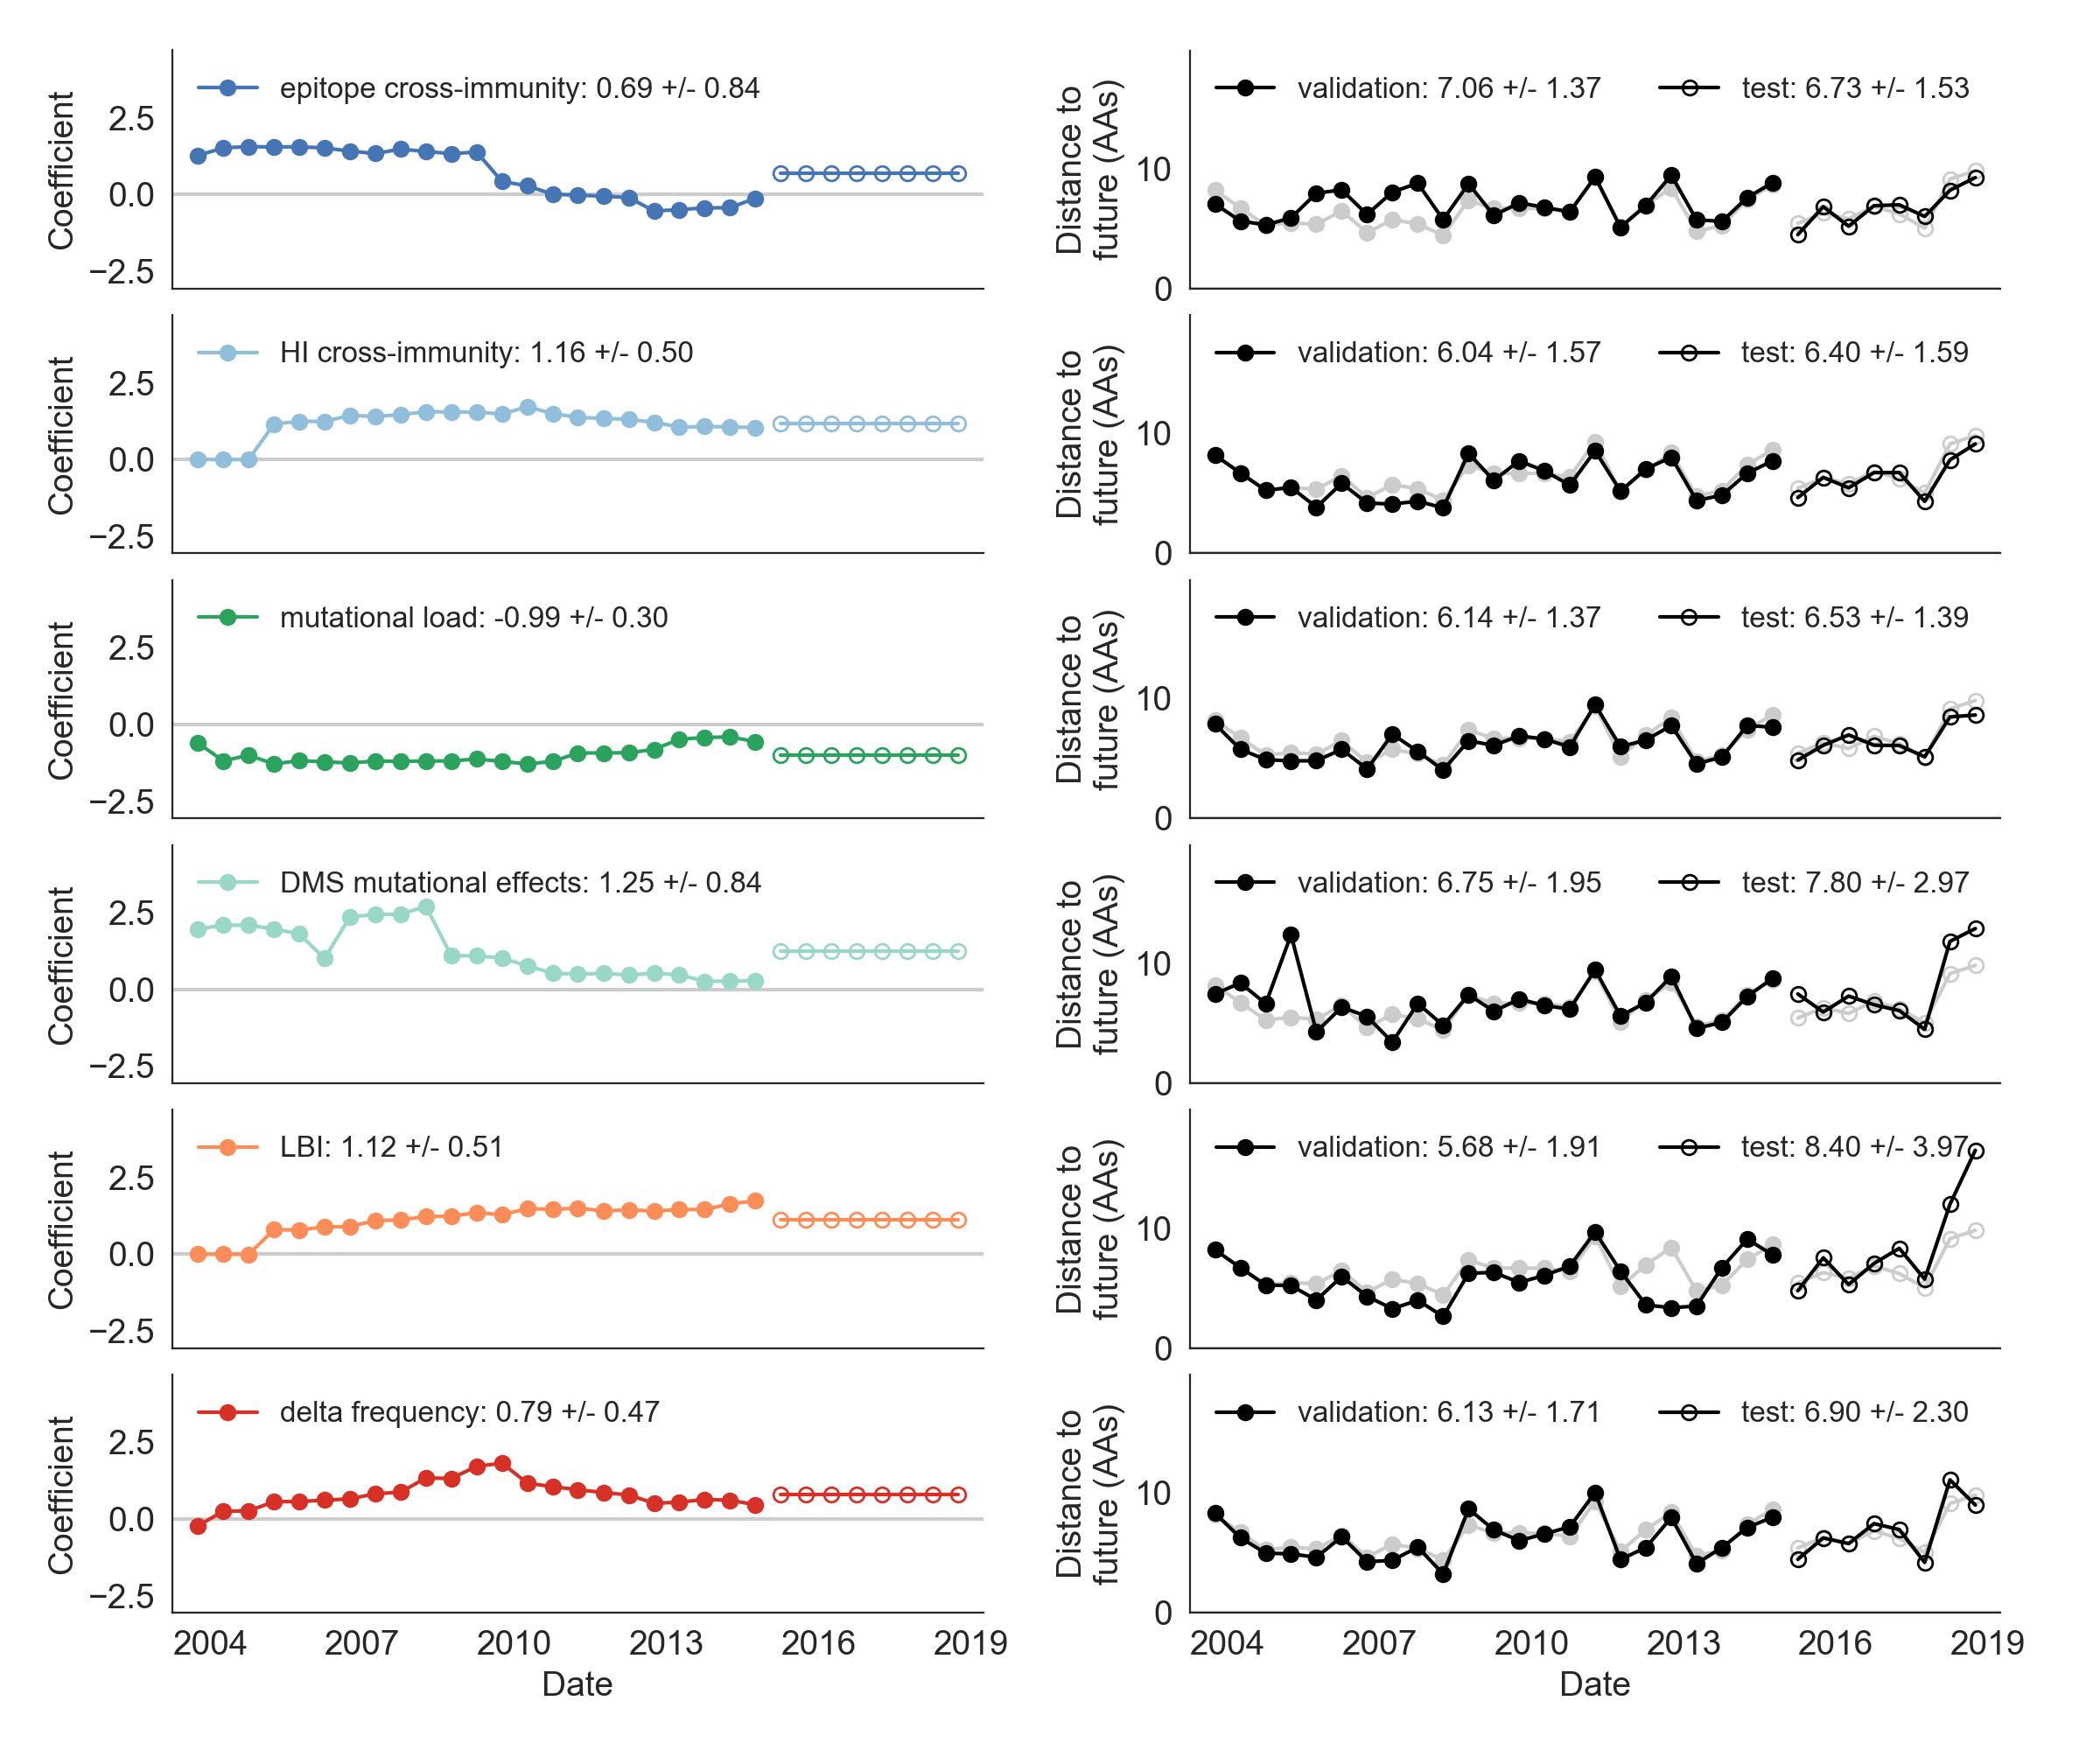
\includegraphics[width=\textwidth]{figures/unadjusted-model-accuracy-and-coefficients-for-natural-populations.png}
  \caption{
    Model a) coefficients and b) distances closer to the future measured in amino acids (AAs) for each model relative to a naive model for natural populations of A/H3N2 viruses.
    As in Fig.~\ref{fig:unadjusted_model_accuracy_and_coefficients_for_simulated_populations}, coefficients are shown for each individual fitness metric per validation timepoint (N=23) in solid circles with the mean $\pm$ standard deviation in the top-left corner of each panel.
    The mean $\pm$ standard deviation of amino acids per validation and test timepoint are shown in the top-left and top-right of each panel, respectively.
  }
  \label{fig:unadjusted_model_accuracy_and_coefficients_for_natural_populations}
  \end{center}
\end{figure*}

\begin{table*}[ht]
  \begin{center}
    
\begin{tabular*}{1.05\textwidth}{lrrrrr}
\toprule
        &                 & \multicolumn{2}{c}{Distance to future (AAs)} & \multicolumn{2}{c}{Model $>$ naive} \\
  Model &    \makecell{Coefficients} & \makecell{Validation} & \makecell{Test} & \makecell{Validation} & \makecell{Test} \\
\midrule

mutational load & -0.68 +/- 0.34 & 5.44 +/- 1.80 & 7.70 +/- 3.53 & 18 (78\%) & 4 (50\%) \\
\hspace{5mm} + LBI & 1.03 +/- 0.40 & & & & \\
LBI & 1.12 +/- 0.51 & 5.68 +/- 1.91 & 8.40 +/- 3.97 & 17 (74\%) & 2 (25\%) \\
HI cross-immunity & 1.39 +/- 0.19 & 5.77 +/- 1.53 & 6.16 +/- 1.43 & 18 (78\%) & 6 (75\%) \\
\hspace{5mm} + mutational load & -1.02 +/- 0.45 & & & & \\
HI cross-immunity & 1.28 +/- 0.47 & 5.88 +/- 1.63 & 6.12 +/- 1.42 & 19 (83\%) & 6 (75\%) \\
\hspace{5mm} + mutational load & -1.03 +/- 0.53 & & & & \\
\hspace{5mm} + LBI & 0.05 +/- 0.50 & & & & \\
HI cross-immunity & 1.16 +/- 0.50 & 6.04 +/- 1.57 & 6.40 +/- 1.59 & 17 (74\%) & 6 (75\%) \\
delta frequency & 0.79 +/- 0.47 & 6.13 +/- 1.71 & 6.90 +/- 2.30 & 16 (70\%) & 5 (62\%) \\
mutational load & -0.99 +/- 0.30 & 6.14 +/- 1.37 & 6.53 +/- 1.39 & 17 (74\%) & 6 (75\%) \\
naive & 0.00 +/- 0.00 & 6.40 +/- 1.36 & 6.82 +/- 1.74 & 0 (0\%) & 0 (0\%) \\
DMS mutational effects & 1.25 +/- 0.84 & 6.75 +/- 1.95 & 7.80 +/- 2.97 & 11 (48\%) & 4 (50\%) \\
epitope cross-immunity & 0.69 +/- 0.84 & 7.06 +/- 1.37 & 6.73 +/- 1.53 & 6 (26\%) & 4 (50\%) \\

\bottomrule
\end{tabular*}

    \caption{
      Model performance with natural A/H3N2 populations relative to the naive model.
      Models use one or more fitness metrics to minimize the distance between the population of HA amino acid sequences at timepoint, $t$, and those at a timepoint one year in the future, $t + 1$.
      The naive model assumes the populations at time $t$ and $t + 1$ are identical, effectively measuring the observed distance between the two timepoints.
      Better models produce estimates that are closer to the future population than the naive model.
    }
    \label{table_natural_model_selection}
  \end{center}
\end{table*}

The average distance per year between natural populations was 6.40 $\pm$ 1.36 amino acids or 71\% of the distance between yearly simulated populations (Supplemental Fig.~\ref{sup_fig:distance_of_natural_populations_between_timepoints}).
Biologically-informed metrics generally performed better than the naive model for natural populations with the exceptions of the epitope cross-immunity and DMS mutational effects (Fig.~\ref{fig:unadjusted_model_accuracy_and_coefficients_for_natural_populations}).
The average improvement of these models over the naive model was consistently lower than the same models in simulated populations.
This reduced performance may be caused by both the reduced diversity between years in natural populations and the increased complexity of the fitness constraints on these real populations.

Surprisingly, the best antigenic fitness metric of HI cross-immunity performed only slightly better the best functional constraint metric of non-epitope mutations.
Indeed, epitope cross-immunity only outperformed the naive model at six of 19 timepoints (26\%), while HI cross-immunity outperformed the naive model at 17 (74\%) timepoints (Table~\ref{table_natural_model_selection}).
Epitope cross-immunity was also the only metric whose coefficient started at a positive value and transitioned to a negative value through the validation period.
This change in coefficient suggests that positive selection may have weakened at these epitope sites over time.
In contrast, HI cross-immunity maintained a positive coefficient across most timepoints.
The HI cross-immunity may benefit from being able to constantly update its antigenic model at each timepoint with recent experimental phenotypes, while the epitope cross-immunity metric is forced to give a constant weight to the same 49 sites throughout time.
Importantly, the 49 epitope sites were originally identified from a historical survey of sites with successful mutations up through 2005 \cite{Shih:2007bd}.
The success of previous epitope models based on these sites could be due to overfitting to these historical data.

Non-epitope mutations also outperformed the DMS mutational effects, reducing the distance to the future by 0.26 $\pm$ 0.56 amino acids on average compared to -0.35 $\pm$ 1.65 amino acids, respectively.
In contrast to the original {\L}uksza and L\"assig \cite{Luksza:2014hj} model, where the coefficient of the non-epitope mutations metric was fixed at -0.5, our model learned a consistently stronger coefficient of -0.99 $\pm$ 0.30.
Notably, the best performance of the DMS mutational effects model was forecasting from April 2007 to April 2008 when the major clade containing A/Perth/16/2009 was first emerging.
This result is consistent with the DMS model overfitting to the evolutionary history of the background strain used to perform the DMS experiments.
Alternate implementations of less background-dependent DMS metrics never performed better than the non-epitope mutations metric (Supplemental Table~\ref{sup_table:complete_natural_model_selection} and Supplemental Fig.~\ref{sup_fig:unadjusted_DMS_model_accuracy_and_coefficients_for_natural_populations}).
Thus, we find that a simple model where any mutation at non-epitope sites is deleterious is more predictive of global viral success than a more comprehensive model based on measured mutational effects.

LBI was the best individual fitness metric by average distance to the future (Fig.~\ref{fig:unadjusted_model_accuracy_and_coefficients_for_natural_populations}) and tied HI cross-immunity and non-epitope mutations for the most timepoints outperforming the naive model of 17 (74\%) (Table~\ref{table_natural_model_selection}).
Delta frequency performed worse than LBI and HI cross-immunity and only performed slightly better than non-epitope mutations.
While delta frequency should, in principle, measure the same aspect of viral fitness as LBI, these results clearly show that the current implementations of these metrics represent qualitatively different fitness components.

\subsection*{Composite models outperform models with individual fitness metrics}

To test whether composite models could outperform individual fitness metrics for natural populations, we fit models based on combinations of best individual metrics representing antigenic drift, functional constraint, and clade growth.
Specifically, we fit models based on HI cross-immunity and non-epitope mutations, LBI and non-epitope mutations, and all three of these metrics together.
We anticipated that if these metrics all represented distinct, mutually beneficial components of viral fitness, these composite models should perform better than individual models with consistent coefficients for each metric.

\begin{figure*}[ht]
  \begin{center}
  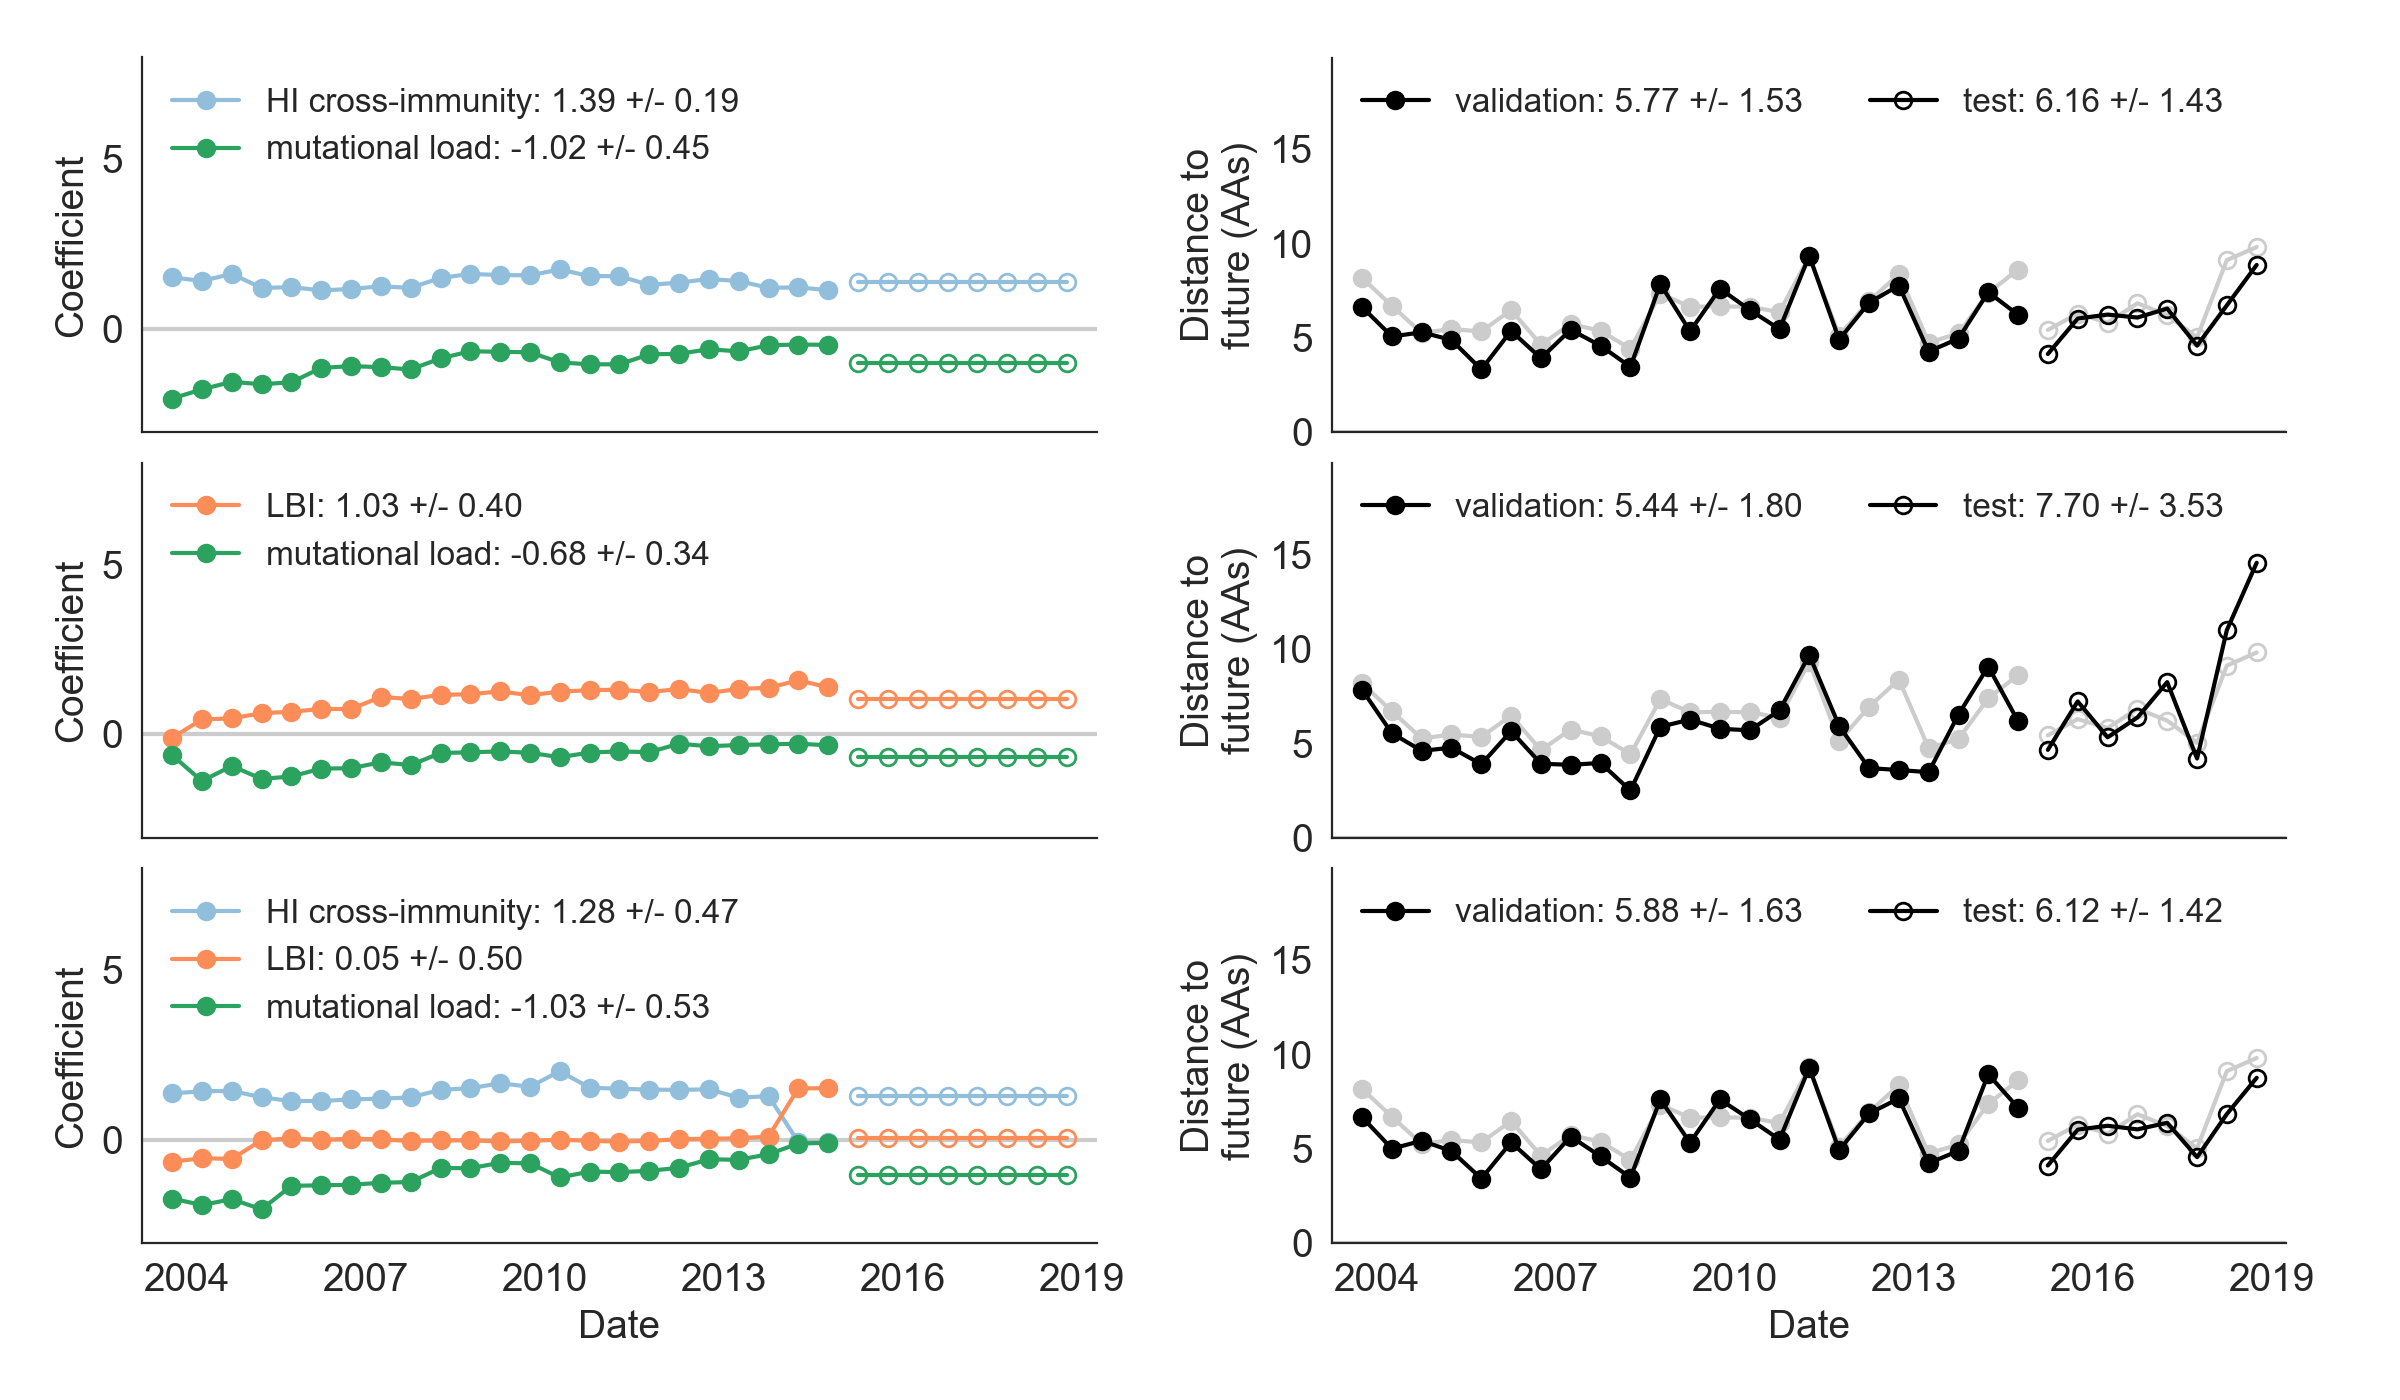
\includegraphics[width=\textwidth]{figures/best-composite-unadjusted-model-accuracy-and-coefficients-for-natural-populations.png}
  \caption{
    Composite model a) accuracy and b) coefficients for natural populations of A/H3N2 viruses.
    As in Fig.~\ref{fig:unadjusted_model_accuracy_and_coefficients_for_natural_populations}, coefficients are shown per timepoint for each individual fitness metric by the corresponding color of the metric.
  }
  \label{fig:unadjusted_composite_model_accuracy_and_coefficients_for_natural_populations}
  \end{center}
\end{figure*}

Both two-metric composite models performed better than their corresponding individual models (Table~\ref{table_natural_model_selection} and Fig.~\ref{fig:unadjusted_composite_model_accuracy_and_coefficients_for_natural_populations}).
Although the three-metric composite model performed slightly worse than the individual LBI model, as measured by distance closer to the future, this composite model outperformed the naive model the most of any model with 19 (83\%) times out of 23.
The composite of LBI and non-epitope mutations performed the best by distance closer to the future at 0.96 $\pm$ 1.42 amino acids.

The stability of the coefficients for the metrics in the two-metric models suggested that these metrics represented complementary components of viral fitness.
In contrast, the three-metric model strongly preferred the HI cross-immunity and non-epitope metrics over LBI for the majority of the validation period, producing an average LBI coefficient of 0.05 $\pm$ 0.50.
In the last two validation timepoints, this composite model converged to a nearly LBI-only model with the coefficients for the other two metrics converging to near-zero values.
These last two timepoints span the period when an HA1:160T substitution swept through the global population.
This substitution introduced a new glycosylation motif and dramatically reduced the efficiency of HI assays \cite{Zost2017}.
These results reinforce the historical importance of HI assays in measuring viral fitness, while also indicating that these assays may no longer be as predictive as sequence-only metrics.

\subsection*{Models enable selection of vaccine candidate strains}

As with the simulated populations, we validated the performance of the best model for natural populations using estimated and observed clade growth rates and the ranking of estimated best strains compared to the observed closest strains to future populations.
The composite model of non-epitope mutations and LBI effectively captured clade growth and decline with 87\% and 89\% accuracy, respectively (Fig.~\ref{fig:validation_of_best_model_for_natural_populations}A).
The estimated best strain from this model was in the top 13th percentile of observed closest strains for half of the validation timepoints and in the top 20th percentile for 70\% of timepoints (Fig.~\ref{fig:validation_of_best_model_for_natural_populations}B).

\begin{figure*}[ht]
  \begin{center}
  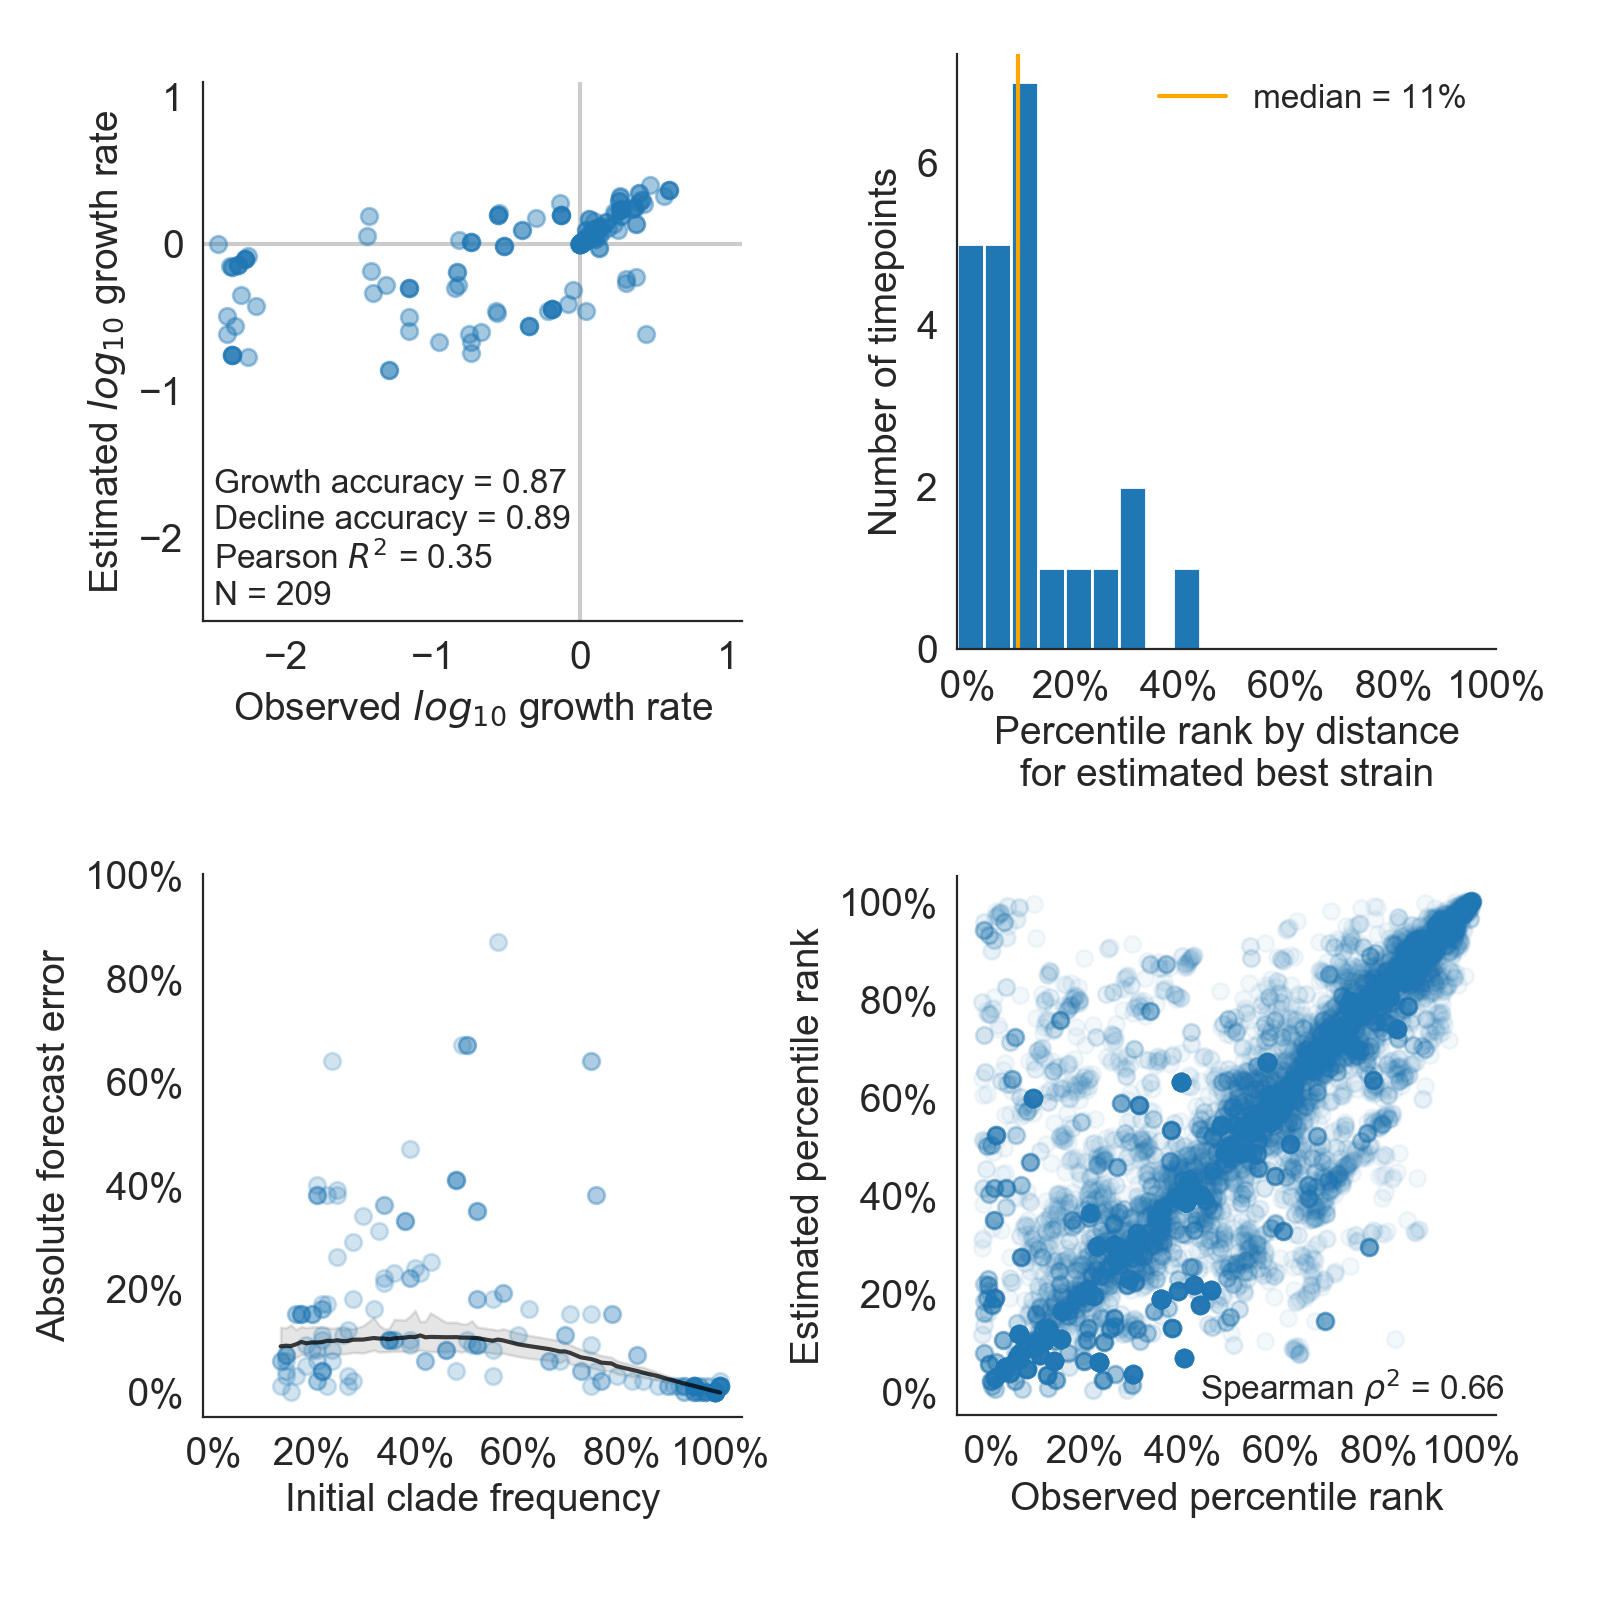
\includegraphics[width=\textwidth]{figures/validation-of-best-model-for-natural-populations.png}
  \caption{
  Validation of best model for natural populations of A/H3N2 viruses, the composite model of non-epitope mutations and LBI.
  A) The correlation of estimated and observed clade growth rates shows the model's ability to capture clade-level dynamics without explicitly optimizing for clade frequency targets.
  B) The rank of the estimated best strain based on its distance to the future in the best model shows how often the model makes a good choice when forced to select a single representative strain for the future population.
  }
  \label{fig:validation_of_best_model_for_natural_populations}
  \end{center}
\end{figure*}

Finally, we tested the performance of this same best model on out-of-sample data collected from October 1, 2015 through April 1, 2019.

\subsection*{Forecasts predict the rise of A1b/131K and A1b/135K sub-clades in September 2020}

After identifying the best model to forecast natural populations, we integrated our forecasting model into our existing open source pathogen surveillance framework, Nextstrain \cite{Hadfield2018}, and used our model to forecast A/H3N2 populations in September 2020.
Our combined non-epitope mutations and LBI model favored the growth of the currently circulating clade A1b/197R, the maintenance of A1b/137F, and the decline of 3c3.A (Fig.~\ref{fig:nextstrain_forecasts}).
To aid with identification of potential vaccine candidates, we annotated samples in the phylogeny by their estimated distance to the future based on our best model (Fig.~\ref{fig:nextstrain_distance_to_future}).

\begin{figure*}[ht]
  \begin{center}
  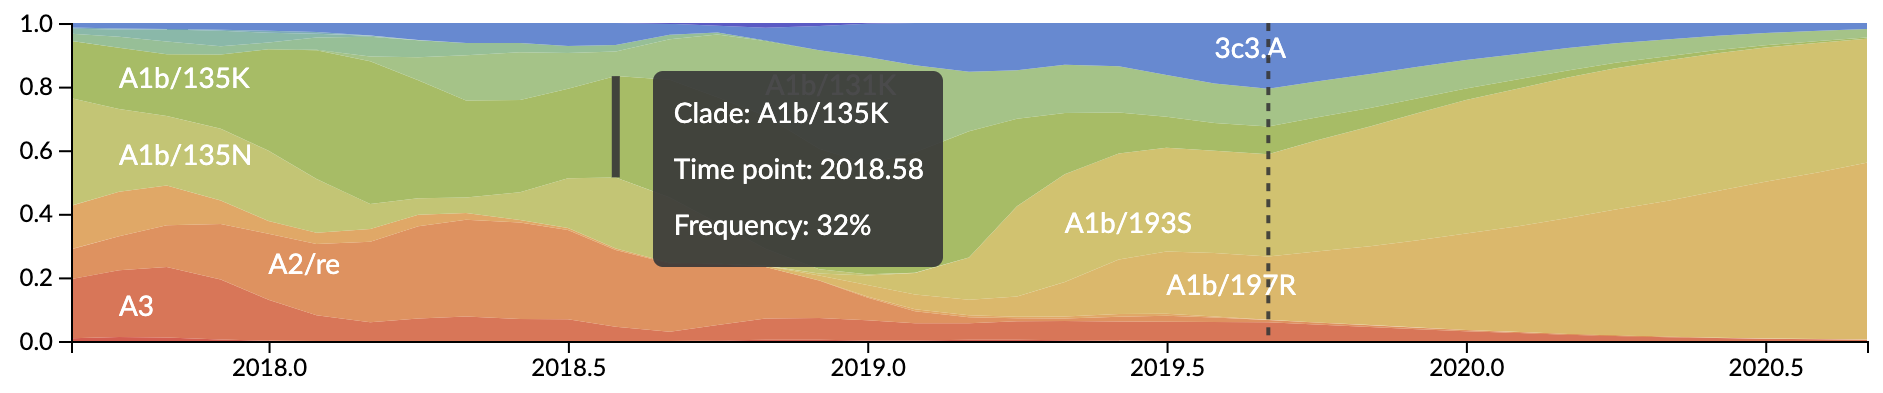
\includegraphics[width=\textwidth]{figures/nextstrain-forecasts-for-september-2020.png}
  \caption{
    Snapshot of live forecasts on nextstrain.org from our best model for September 2020.
    The observed frequency trajectories for currently circulating clades are shown up to September 2019.
    Our model favors the A1b/131K subclade, A1b/197R, to grow over the next year and estimates that the A1b/135K subclade, A1b/137F, will remain stable.
  }
  \label{fig:nextstrain_forecasts}
  \end{center}
\end{figure*}

\begin{figure*}[ht]
  \begin{center}
  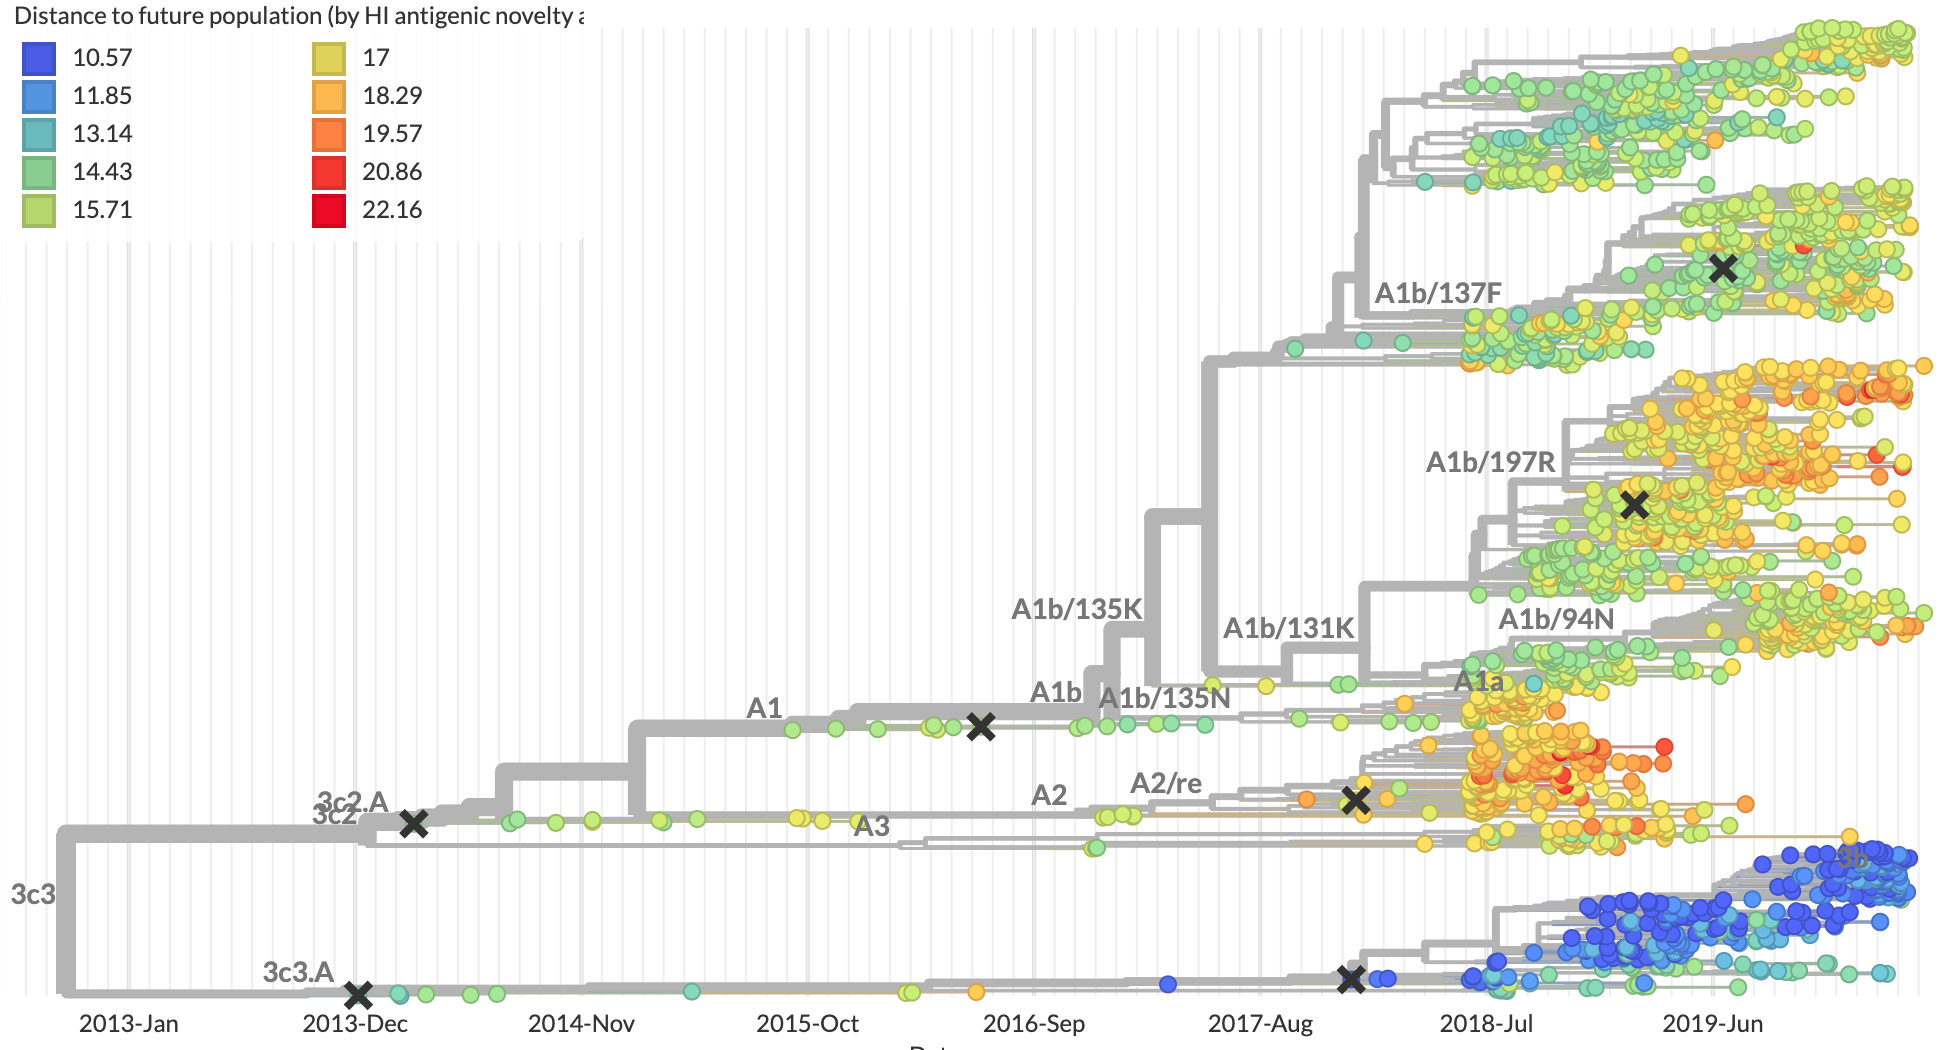
\includegraphics[width=\textwidth]{figures/nextstrain-weighted-distance-to-future-per-strain.png}
  \caption{
    Snapshot of the last two years of seasonal influenza A/H3N2 evolution on nextstrain.org showing the estimated distance per sample to the future population.
    Distance to the future is calculated for each sample as the Hamming distance of HA amino acid sequences to all other circulating samples weighted by the other sample's projected frequencies under the best fitness model.
  }
  \label{fig:nextstrain_distance_to_future}
  \end{center}
\end{figure*}

\section*{Discussion}

Key findings:

\begin{itemize}
\item{Our model accurately forecasts clade frequency trajectories and identifies optimal potential vaccine strains for both simulated and natural populations by estimating the sequence composition of future populations and without relying on clade-based model targets}
\item{Experimental measurements of antigenic drift based on HI assays are more predictive of viral success than epitope mutations}
\item{The combination of sequence-only metrics outperforms all experimentally-informed metrics}
\item{Deleterious mutations contribute more to seasonal influenza evolution than has been as widely appreciated}
\item{DMS measurements appear to be too background-specific to be predictive for global viral success}
\item{Further efforts to understand the declining efficacy of HI assays and to replace these with FRA or antigenic escape assays could improve models in the future}
\item{Our model live forecasts in nextstrain.org will aid in year-round surveillance of influenza evolutionary patterns and allow us to continuously evaluate model performance relative to recent observations}
\item{Our model is the first of its kind to be released as an open source framework that can be inspected and extended by others}
\item{Immediate next steps to improve influenza models under this framework include the integration of geographic information and antigenic escape assay data}
\item{Our distance-based model targets and easy definition of fitness metrics through tidy data frames paves the way for future forecasting efforts with pathogens that cannot be analyzed by standard phylogenetic methods (e.g., highly recombinant viruses and organisms with larger genomes like bacteria and fungi)}
\end{itemize}

\section*{Methods}

\subsection*{Simulation of influenza A/H3N2-like populations}

We simulated the long-term evolution of A/H3N2-like viruses with SANTA-SIM \cite{Jariani2019} for 50 years where 200 generations was equivalent to 1 year.
We discarded the first 10 years as a burn-in period, selected the next 30 years for model fitting and validation, and held out the last 10 years as out-of-sample data for model testing.
Each simulated population was seeded with the full length HA from A/Beijing/32/1992 (NCBI accession: U26830.1) such that all simulated sequences contained signal peptide, HA1, and HA2 domains.
We defined purifying selection across all three domains, allowing the preferred amino acid at each site to change at a fixed rate over time.
We additionally defined exposure-dependent selection for 49 putative epitope sites in HA1 \cite{Luksza:2014hj} to impose an effect of cross-immunity that would allow mutations at those sites to increase viral fitness despite underlying purifying selection.
We modified the SANTA-SIM source code to enable the inclusion of true fitness values for each sample in the FASTA header of the sampled sequences from each generation.
This modified implementation is available at \url{https://github.com/huddlej/santa-sim/tree/emit-fitness}.
For our full analysis of model performance, we sampled 90 viruses per month to match the sampling density of natural populations.
For tuning of hyperparameters, we sampled 10 viruses per month to enable rapid exploration of hyperparameter space.

\subsection*{Hyperparameter tuning with simulated populations}

To avoid overfitting our models to the relatively limited data from natural populations, we used simulated A/H3N2-like populations to tune hyperparameters including the KDE bandwidth for frequency estimates and the L1 penalty for model coefficients.
We simulated populations, as described above, and fit models for each parameter value using the true fitness of samples from the simulator.

We identified the optimal KDE bandwidth for frequencies as the value that minimized the difference between the mean distances to the future from the true fitness model and the naive model.
We set the L1 lambda penalty to zero, to reduce variables in the analysis and avoid interactions between the coefficients and the KDE bandwidths.
Higher bandwidths completely wash out dynamics of populations by making all samples appear to exist for long time periods.
This flattening of frequency trajectories means that as bandwidths increase, the naive model gets more accurate and less informative.
Given this behavior, we found the bandwidth that produced the minimum difference between distances to the future for the true fitness and naive models instead of the bandwidth that produced the minimum mean model distance.
Based on this analysis, we identified an optimal bandwidth of $\frac{2}{12}$ or the equivalent of 2-months for floating point dates.
Next, we identified an L1 penalty of 0.1 for model coefficients that minimized the mean distance to the future for the true fitness model.

\subsection*{Strain selection for natural populations}

For model training and validation, we selected 13,601 HA sequences $\geq$900 nucleotides that were sampled between October 1, 1990 and October 1, 2015.
To account for known variation in sequence availability by region, we subsampled the selected sequences to a representative set of 90 viruses per month with even sampling across 10 global regions including Africa, Europe, North America, China, South Asia, Japan and Korea, Oceania, South America, Southeast Asia, and West Asia.
We excluded all egg-passaged samples and all samples with ambiguous year, month, and day annotations.
We prioritized samples with more available HI titer measurements.
For model testing, we selected an additional 20,719 HA sequences corresponding to 90 viruses per month sampled between October 1, 2015 and October 1, 2019.
This increased number of sequences corresponds with the trend of increased sample sequencing and deposition in the last decade.
We used these test sequences to evaluate the out-of-sample error of fixed model parameters learned during training and validation.

\subsection*{Phylogenetic inference}

For each timepoint in model training, validation, and testing, we selected the subsampled HA sequences with collection dates up to that timepoint.
We aligned sequences with the augur align command \cite{Hadfield2018} and MAFFT v7.407 \cite{Katoh2002}.
We inferred initial phylogenies for HA sequences at each timepoint with IQ-TREE v1.6.10 \cite{Nguyen2014}.
To reconstruct time-resolved phylogenies, we applied TreeTime v0.5.6 \cite{Sagulenko2018} with the augur refine command.

\subsection*{Frequency estimation}

To account for uncertainty in collection date and sampling error, we applied a kernel density estimation (KDE) approach to calculate global sample frequencies.
Specifically, we constructed a Gaussian kernel for each sample with the mean at the reported collection date and a variance (or KDE bandwidth) of two months.
The bandwidth was identified by cross-validation, as described above.
This bandwidth also roughly corresponds to the median lag time between sample collection and submission to the GISAID database.
We estimated the frequency of each sample at each timepoint by calculating the probabilitiy density function of each KDE at that timepoint and normalizing the resulting values to sum to one.
We implemented this frequency estimation logic in the augur frequencies command.

\subsection*{Model fitting and evaluation}

\subsubsection*{Fitness model}

We assumed that the evolution seasonal influenza A/H3N2 populations can be represented by a Malthusian growth fitness model, as previously described \cite{Luksza:2014hj}.
Under this model, we estimated the future frequency of the global population, $\mathbf{\hat{x}}$, at some time in the future, $t + \Delta{t}$, based on the current frequency, $x_{i}(t)$, and fitness, $f_{i}(t)$, of each sample $i$ as follows where the resulting future frequencies were normalized to one by $\frac{1}{Z(t)}$.

\begin{equation}
    \mathbf{\hat{x}}(t + \Delta{t}) = \frac{1}{Z(t)}\sum_{i}x_{i}(t)\exp(f_{i}(t)\Delta{t})
    \label{equation_exponential_growth_model}
\end{equation}

We defined the fitness of each sample at time $t$ as the additive combination of one or more fitness metrics, $f_{i,m}$, scaled by fitness coefficients, $\beta_{m}$.
For example, Equation~\ref{equation_fitness_estimation} estimates fitness per sample by non-epitope mutations ($\mathrm{ne}$) and local branching index ($\mathrm{lbi}$).

\begin{equation}
    f_{i}(t) = \beta_{\mathrm{ne}}f_{i, \mathrm{ne}}(t) + \beta_{\mathrm{lbi}}f_{i, \mathrm{lbi}}(t)
    \label{equation_fitness_estimation}
\end{equation}

\subsubsection*{Model target}

For a model based on any given combination of fitness metrics, we found the fitness coefficients that minimized the weighted Hamming distance between amino acid sequences from the observed future population at time $u = t + \Delta{t}$ and the estimated future population created by projecting frequencies of samples at time $t$ by their estimated fitnesses.
We measured distance between populations using Earth Mover's Distance (EMD), a metric commonly applied in machine learning to compare collections of pixels or words \cite{Rubner1998,Kusner2015}.
Solving for EMD identifies the minimum about of ``earth'' that must be moved from a source population to a sink population to make those populations as similar as possible.
This solution requires both a ``ground distance'' between pairs fo samples from both populations and weights assigned to each sample that determine how much that sample contributes to the overall distance.

For each timepoint $t$ and corresponding timepoint $u = t + 1$, we defined the ground distance as the Hamming distance between HA amino acid sequences for all pairs of samples between timepoints.
For samples with less than full length nucleotide sequences, we inferred missing nucleotides through TreeTime's ancestral sequence reconstruction analysis.
We defined weights for samples at timepoint $t$ based on their projected future frequencies.
We defined weights for samples at timepoint $u$ based on their observed frequencies.
We then identified the fitness coefficients that provided projected future frequencies that minimized the EMD between the estimated and observed future populations.
With this metric, an optimal estimate of the future would produce a distance of zero.
However, the inevitable accumulation of substitutions between the two populations prevents this outcome.
We calculated EMD with the Python bindings for the OpenCV 3.4.1 implementation \cite{opencv_library}.
We applied the Nelder-Mead minimization algorithm as implemented in SciPy \cite{SciPy} to learn fitness coefficients that minimize the average of this distance metric over all timepoints in a given training window.

\subsubsection*{Time-series cross-validation}

To obtain unbiased estimates for the out-of-sample errors of our models, we adopted the standard cross-validation strategy of training, validation, and testing.
We divided our available data into an initial training and validation set spanning October 1990 to October 2015 and an additional testing set spanning October 2015 to April 2019.
We partitioned our training and validation data into six month seasons corresponding to winter in the Northern Hemisphere (October--April) and the Southern Hemisphere (April--October) and trained models to estimate frequencies of populations one year into the future from each season in six-year sliding windows.
To calculate validation error for each training window, we applied the resulting model coefficients to estimate the future frequencies for the year after the last timepoint in the training window.
These validation errors informed our tuning of hyperparameters including a L1 regularization of the fitness coefficients, the LBI neighborhood parameter $\tau$, and the length of the training window itself.
Finally, we fixed the coefficients for each model at the mean values across all training windows and applied these fixed models to the test data to estimate the true forecasting accuracy of each model on previously unobserved data.

\subsection*{Fitness metrics}

We defined the following fitness metrics per strain and timepoint.

\subsubsection*{Antigenic drift}

We estimated antigenic drift for each strain using either genetic or HI data.
To estimate antigenic drift with genetic data, we implemented the cross-immunity metric originally defined by {\L}uksza and L\"assig \cite{Luksza:2014hj}.
Briefly, for each pair of strains in adjacent seasons, we counted the number of amino acid differences between the strains' HA sequences at 49 epitope sites.
The one-based coordinates of these sites relative to the start of the HA1 segment were 50, 53, 54, 121, 122, 124, 126, 131, 133, 135, 137, 142, 143, 144, 145, 146, 155, 156, 157, 158, 159, 160, 163, 164, 172, 173, 174, 186, 188, 189, 190, 192, 193, 196, 197, 201, 207, 213, 217, 226, 227, 242, 244, 248, 275, 276, 278, 299, and 307.
We limited pairwise comparisons to all strains sampled within the last five years from each timepoint.
For each individual strain $i$ at each timepoint $t$, we estimated that strain's ability to escape cross-immunity by summing the exponentially-scaled epitope distances between previously circulating strains and the given strain as follows.

\begin{equation}
    f_{i,\mathrm{ep}}(t) = \sum_{j: t_{j} < t_{i}}{x_{j}\exp{(-D_{\mathrm{ep}}(a_{i}, a_{j}) / D_{0})}}
    \label{equation_epitope_cross_immunity}
\end{equation}

To estimate antigenic drift with HI data, we first applied the titer tree model to the phylogeny at a given timepoint and the corresponding HI data for its strains, as previously described by Neher et al. 2016 \cite{Neher:2016hy}.
This method effectively estimates the antigenic drift per branch in units of $log_{2}$ titer change.
Next, we calculated the pairwise antigenic distance between strains as the sum of antigenic drift weights per branch on the phylogenetic path between each pair of strains.
Finally, we calculated each strain's ability to escape cross-immunity using Equation~\ref{equation_epitope_cross_immunity} with the pairwise distances between epitope sequences replaced with pairwise antigenic distance from HI data.
As with the original epitope cross-immunity described above, this HI cross-immunity metric produces higher values for strains that are more antigenically distinct from previously circulating strains.

\subsubsection*{Functional constraint}

We estimated functional constraint for each strain using either genetic or deep mutational scanning (DMS) data.
To estimate functional constraint with genetic data, we implemented the non-epitope mutation metric originally defined by {\L}uksza and L\"assig \cite{Luksza:2014hj}.
This metric counts the number of amino acid differences at 517 non-epitope sites in HA sequences between each strain $i$ at timepoint $t$ and that strain's most recent inferred ancestral sequence in the previous season ($t - 1$).

We estimated functional constraint using mutational preferences from DMS data as previously defined \cite{Lee2018}.
Briefly, mutational effects were defined as the log ratio of DMS preferences, $\pi$, at site $r$ for the derived amino acid, $a_{i}$, and the ancestral amino acid, $a_{j}$.
As with the non-epitope mutation metric above, we considered only substitutions in HA between each strain $i$ and that strain's most recent inferred ancestral sequence in the previous season.
We calculated the total effect of these substitutions as the sum of the mutational preferences for each substitution, as in Equation~\ref{equation_mutational_preference}.

\begin{equation}
    f_{i,\mathrm{DMS}}(t) = \sum_{r \in r,a_{i} != r,a_{j}}\log_{2}\frac{\pi_{r,a_{i}}}{\pi_{r,a_{j}}}
    \label{equation_mutational_preference}
\end{equation}

\subsubsection*{Clade growth}

We estimated clade growth for each strain using local branching index (LBI) and the change in frequency over time (delta frequency).
To calculate LBI for each strain at each timepoint, we applied the LBI heuristic algorithm as originally described \cite{Neher:2014eu} to the phylogenetic tree constructed at each timepoint.
We set the neighborhood parameter, $\tau$, to 0.3 and only considered viruses sampled in the last 6 months of each phylogeny as contributing to recent clade growth.

We estimated the change in frequency over time by calculating clade frequencies under a Brownian motion diffusion process as previously described \cite{Lee2018}.
These frequency calculations allowed us to assign a partial clade frequency to each strain within nested clades.
We calculated the delta frequency as the change in frequency for each strain between the most recent timepoint in a given phylogeny and six months prior to that timepoint divided by 0.5 years.
